\documentclass[journal]{./template/IEEEtran}
\IEEEoverridecommandlockouts
\usepackage{cite}
\usepackage{amsmath,amssymb,amsfonts}
\usepackage[caption=false]{subfig}
%\usepackage{subcaption}
\usepackage{algorithm}
\usepackage{algorithmic}
\usepackage{graphicx}
\usepackage{textcomp}
\usepackage{xcolor}
\usepackage{url}
\usepackage{comment}
\usepackage{multirow}
\usepackage{commath}
\usepackage[utf8]{inputenc}
\usepackage{kotex}
\usepackage{epstopdf}
\def\BibTeX{{\rm B\kern-.05em{\sc i\kern-.025em b}\kern-.08em
    T\kern-.1667em\lower.7ex\hbox{E}\kern-.125emX}}
\usepackage{amssymb}% http://ctan.org/pkg/amssymb
\usepackage{pifont}% http://ctan.org/pkg/pifont
\newcommand{\cmark}{\ding{51}}%
\newcommand{\xmark}{\ding{55}}%
%\renewcommand{\bottomfraction}{0.9}
\begin{document}

\makeatletter

\newcommand\blfootnote[1]{%
  \begingroup
  \renewcommand\thefootnote{}\footnote{#1}%
  \addtocounter{footnote}{-1}%
  \endgroup
}

\newcommand\fs@norules{\def\@fs@cfont{\bfseries}\let\@fs@capt\floatc@ruled
  \def\@fs@pre{}%
  \def\@fs@post{}%
  \def\@fs@mid{\kern3pt}%
  \let\@fs@iftopcapt\iftrue}
\makeatother
\floatstyle{norules}
\restylefloat{algorithm}

\title{Least-Energy Path Planning With Building Accurate Power Consumption Model of Rotary Unmanned Aerial Vehicle\\
}
\author{
Dooyoung Hong,\,\IEEEmembership{Student Member,\,IEEE,}
Seonhoon Lee,\,\IEEEmembership{Student Member,\,IEEE,}\\
Jaemin Kim*,\,\IEEEmembership{Member,\,IEEE,}
Naehyuck Chang*,\,\IEEEmembership{Fellow,\,IEEE,}
\thanks{Direct questions and comments about this article to Jaemin Kim, Myongji University, 116 Myongji-ro, Cheoin-gu, Yongin, Korea\, (e-mail: jaemin@esl.mju.ac.kr) and Naehyuck Chang, Korea Advanced Institute of Science and Technology, 291, Daehak-ro, Yuseong-gu, Daejeon, Korea (e-mail: naehyuck@cad4x.kaist.ac.kr).}
}
\maketitle
\blfootnote{* Corresponding Authors}

\begin{abstract}

Rotary Unmanned Aerial Vehicles (UAVs), also known as drones, have advantages in various aspects, yet the actual applications are limited due to the flight range. However, it is challenging to increase the flight range through enhancement of the hardware. 
In this paper, we introduce the first step of systematic drone low-power run-time optimization in the framework of electronic design automation (EDA). 
We attempt the drone power management without in-depth knowledge of aerodynamics and control theory. 
Instead, we introduce a novel power modeling of drones using physical parameters that can affect power consumption such as three-axis velocity and acceleration, the height of drones, wind velocity, the weight and volume of the load. 
This paper presents a detailed experimental setup, power modeling, accuracy verification, and optimization for energy minimum path. 
We achieved over 90\,\% accuracy in power modeling without depending on the aerodynamics. 
The proposed approach shows the feasibility of energy-aware rotary UAV flight trajectory optimization considering the external forces that affect drones such as wind. The proposed method presents up to 12.7\,\% energy saving.
\label{Section: abstract}
\end{abstract}














\section{Introduction}
\label{Section: introduction}

The unmanned aerial vehicles (UAVs) are equipped with fixed-wings or rotor wings.
The fixed-wing methods gain the lift generated by the pressure difference between the upper and lower sides of the wings when the aircraft moves forward. 
On the other hand, the rotor wing method exploits the thrust produced by multiple motors and propellers. Generally, UAVs using the rotor wing method are called drones. Unlike the fixed-wing UAVs, drones can take off and land without the restriction of space. 
Modern drones have a built-in flight assistance controller, so even novices can easily control the drones. 
In this paper, we focus on the rotor wing UAVs: drones. 
Drones can be equipped with internal combustion engines or batteries as the propulsion power source. However, we narrow down the focus to the battery-operated drones.
Battery-powered drones have various distinct advantages such as zero emission, low noise, and ease of controllability.
Despite those advantages, one of the biggest challenges and limitations of the battery-operated drones is the flight range and time. 
The flight range and time limitation come primarily from the battery energy density, i.e., the energy capacity per unit weight.
In other words, it is hard to scale the flight range and time by simply installing higher capacity batteries as the battery weight also increases linearly by the capacity. 
The weight of the battery is one of the most critical factors for the power consumption of drones. 
Many previous studies have addressed insufficient flight time of drones. 
These efforts aim to increase the flight time through the development of hardware such as motors and batteries\,\cite{ref_1}.
Such a component-based approach has led the evolution of drones, but such practices are being matured exhibiting above 90\,\% efficiency\,\cite{ref_2}, which eventually will lose the driving force of drone evolution. 

In this work, we introduce a system-level approach to enhance flight range and time of drones.
Such an approach is not fundamentally new, but to our knowledge, we are the first to attempt a systematic framework {inspired by} electronic design automation (EDA) technique as used in the design process of semiconductors.
We have elaborated on the power consumption model of drones, characterized the power model with the actual flight data of the drone, considering the effect of external elements such as wind and the payload weight, and constructed an accurate simulator.
In order to construct the Accurate power consumption model based on the actual drone data, we figure out the power consumption characteristics of a top-of-the-line commercial drone through dozens of hours of power measurement both on the air and ground.
We develop a high precision onboard drone power measurement system not to negotiate the measurement fidelity by not using the built-in power measurement feature. 
The power consumption of the drone has been accurately measured using the power measurement board, and a navigation and positioning assistance system called real-time kinetic global navigation satellite system (RTK GNSS), which supports the drones global positioning system (GPS), is installed to collect precise flight status data of drones.
We also equip a wind sensor capable of measuring 360 degrees of wind velocity to measure the additional power consumption of drones caused by wind effects during the flight.
Following the systematic framework we proposed, we try various ways of data analysis and modeling, and we develop a power consumption model using deep learning that can predict power consumption using simple variables that represent the power consumption of the drone without a problematic understanding of aerodynamics.
As a result, we develop the power consumption model that has less than 10\,\% error, which has been verified with a high precision data acquisition device.
The proposed power model can be easily plugged in linear programming, dynamic programming, and Reinforcement Learning (RL) that have been intensely studied to optimize complex design problems with the approximation within a given time complexity.
Such an effort becomes a basis for the systematic optimization of drones.
This paper not only focuses on power measurement, modeling, and characterization, but we also demonstrate the optimization method of drones to find the energy-efficient flight paths in a given mission, and we verify the derived energy-efficient paths through the actual flight experiments.
Finally, we present an example of a complicated drone energy optimization using the Dijkstra algorithm to derive an energy-optimized route to the destination in given scenarios with various obstacles imparted by wind fields.









\section{Related work}

Previously, drone power management focuses on finding the optimal route between the destinations when a mission of drone is given.
Such practices require to develop the power or energy consumption model first. 
Related literature develops either a theoretical model or a data-driven model from flight experiment data. 
Each modeling derives the parameters necessary for each model through the specification or data measurement of drones and uses them for model formation.
The power consumption model based on the theories can describe the flight of aircraft as a physical phenomenon, expressing the principle of power consumption as a force in a horizontal direction and a force for rotation, to clearly express the factors affecting the power consumption.
For example, some researchers focus on aerodynamic characteristics of drones.
They analyze the power consumption due to the propeller drag and the movement of the drone based on fluid mechanics and dynamics\,\cite{ref_3}.
However, coefficients for expressing theoretical forces (e.g., air resistance, motor efficiency, and propeller efficiency) cannot be obtained by simple measurements. 
Since the coefficients and specifications of non-measurable drone parameters only depend on the information provided by the manufacturer of the component, the power consumption of the model based on this information may differ from the actual power usage.
In addition, the aerodynamic-based model cannot directly consider the disturbance that has a huge impact on the power consumption of drones during the actual flight.
Therefore, there is a difference between the power consumption measured in actual flight and the power consumption predicted by the aerodynamics model.
On the contrary, the model using the momentum theory that infers the power consumption from the thrust of motor and the propeller has very high accuracy because the power consumption and the power source are directly related, but the momentum theory is only valid for the calculation of the thrust with hovering state of drones. 
It is difficult to apply to drones that must fly in multiple directions to perform\,\cite{ref_4}.
Those who construct theoretical power consumption models use the traditional power consumption model for hovering rotor-crafts\,\cite{ref_4}, or they use the relationship between the thrust and revolutions per minute (RPM) of the propeller\,\cite{ref_5}. 
It is straightforward to relate the power consumption of drones with the motor torque, current, RPM, and supplied voltage\,\cite{ref_6,ref_7}.

Although the data-driven modeling method requires a lot of actual measurement data to build the model, the constructed model has high accuracy if the collected amount of data is a lot and accurate enough.
As a white- to gray-box power modeling, the characterization starts from known actual data of drones. 
The data-driven model can accurately predict the power consumption of a drone without knowledge of aerodynamics or complicated calculations if the variables that can highly affect the power consumption (e.g., velocity, acceleration, disturbance, etc.) are properly selected as the inputs of the model.
For example, C. D. Franco analyzes that the relationship of the power consumption and the velocity of the drone based on a experimental flight data\,\cite{ref_8}.  
However, The model assumes that the power consumption for ascending, descending and hovering is constant. Thus, the model is lack of accuracy.
In\,\cite{ref_9}, a linear regression model is used to estimate the power consumption for a quad-rotor using onboard power measurement functions. 
However, this causes significant misleading in power modeling according to our measurement.
The data from the factory onboard power measurement of commercial drones is not accurate enough; the resultant power models can potentially impractical and cause false predictions.

Based on the power or energy consumption model of drones, many studies try to broaden the operation area of drones by minimizing the energy consumption of drones.
In other words, the studies utilize optimization algorithms to minimize the energy consumption of drones and to optimize flight paths to achieve a given purpose or to minimize flight time.
In order to solve the optimization of drones by the numerical method, the studies optimize the total energy over time by using the control variables along with the power model. 
N. Bezzo et al propose Energy-aware planning\,\cite{ref_5}. The Model Predictive Controller is used to determine the desired control inputs of the non-linear power consumption model of Helicopter theory that fan thrust is proportional to the square of RPM.
The optimal energy control system derives the minimum energy path through the mathematical solution using the Sequential quadratic programming (SQP) algorithm\,\cite{ref_6}. 
In\,\cite{ref_6}, the model of the control system uses the voltage and torque of the drone motor and the dynamic equations of the drone. 
On the other hand, F. Yacef et al derive the optimal path using the Legendre-Gauss-Radau (LGR) orthogonal collocation method that the numerical algorithm using the motor torque and RPM as major factors affecting the power efficiency and battery life\,\cite{ref_7}. 
The optimization of the drone using the numerical algorithm is good for expressing continuous movements, but it cannot reveal unexpected environment variables, which should be measured directly.

\begin{table*}[ht]
\caption{Comparison of Previous Works for Drone Optimization.}
\label{Table: survay_result}
\centering
\begin{tabular}{|c|c|c|c|c|c|}
\hline
Reference Paper & Wind & Payload & Surface area & Optimization method & Goal \\ \hline
%TVLSI 2019 & \cmark & \cmark & \cmark & Dijkstra algorithm & \multicolumn{1}{l|}{Minimum energy} \\ \hline
ICARSC 2015 {[}7{]} & %\xmark 
& %\xmark 
& %\xmark 
& Back-and-forth algorithm & Minimum energy \\ \hline
IROS 2016 {[}5{]} & \cmark & %\xmark 
& %\xmark 
& Model predictive control & Minimum energy \\ \hline
ICRA 2016 {[}6{]} & %\xmark 
& \cmark & %\xmark 
& SQP algorithm & Minimum energy \\ \hline
IMAV 2017 {[}8{]} & %\xmark 
& \cmark & \cmark & LGR orthogonal collocation & Minimum energy \\ \hline
SysCon 2017 {[}10{]} & \cmark & %\xmark 
& %\xmark 
& Fast marching method & Minimum energy \\ \hline
arXiv 2017 {[}9{]} & \cmark & \cmark & %\xmark 
& Dynamic graph algorithm &Shortest time \\ \hline
\end{tabular}
\end{table*}

On the other hand, the studies to solve the optimization of drones using the graph search algorithm are optimized by finding a path of drone that minimizes the power consumption as the drone moves according to each step set in the graph. 
The graph search algorithm is easy to implement the fields and constraints on which the drones can move, and can easily calculate the long-term operation of drones in the implemented graph.
However, since the movement of drone is limited to each step of the graph, it is difficult to infer the continuous movement of the drone in the step, and it is also difficult to calculate the high dimension that can’t be visualized.
So that, previous studies use the heuristic to fix speed or direction to reduce dimensions.
The heuristic that fixes the speed and direction limits the degree of freedom of drones and adversely affects the results of optimization due to limited movement.
Z. Lui focuses on deriving the optimal path using the fast marching method, a variant of the Dijkstra algorithm, and a flight endurance model based on hovering power consumption and battery model\,\cite{ref_10}.
Unlike the previous papers, \cite{ref_8,ref_9} established and optimized power consumption model based on the regression method using the actual drone data.
Authors measured the power consumption and the speed of drones through experiments \cite{ref_8}. They also expressed the power consumption as a function of speed to derive an energy-efficient aerial flight path using Back-and-forth algorithm.
In\,\cite{ref_9}, the power consumption is established as a multivariate regression model based on the data measured through actual flight experiments of the drone.
The minimum time path is also derived by considering the battery recharging in the case of multiple destinations. 
We briefly summarize the literature in Table\,\ref{Table: survay_result}, which shows the factors considered for optimization in each study, the algorithms used for the optimization, and the goals of the optimization.

\label{Section: Related works}









\section{Motivation}




\subsection{Problem statement}

Our goal is to minimize the total energy consumption of the drone with given missions by the least energy path planning.
Different types of drones can be given depending on the number of motors and the size of the body frame, and the starting and finishing points, weight and volume of payload, and three-dimensional geographic data are also given as a mission.
In order to achieve our goal, we divide the least energy path planning problem of the drone into two sub-problems.
The first sub-problem consists of securing the power consumption data and the flight data of the drone, which are used to build an accurate power consumption model.
Even though almost all of the commercially available drone presents logs and shows the flight data such as battery voltage, battery current, flight speed, and so on, but the data is not guaranteed to be accurate. We first build an accurate power model with accurate flight data with our own measurement system.
The second sub-problem consists of inferring the path that the drone consumes the least energy to the target point within a given mission and finding the path changed by external forces using the delivered accurate drone power model from the first sub-problem. 
We formulate three-dimensional geographic data into a three-dimensional discrete node array by assuming that the drone determines to change its speed, considering the acceleration, and posture at each node.
We present the problem of least energy path planning in the following:

\vspace{5pt}
\hrule
\vspace{5pt}
\noindent\textit{\textbf{Least Energy Path Planning Problem Statement}}
~\\
\noindent\textit{\textbf{Given:}} The drone with various types, Starting and finishing points of the drone (mission), Weight and volume of payload, Three-dimensional geographic data of mission area.
~\\
\noindent\textit{\textbf{Control knob:}} The drone movement.
~\\
\noindent\textit{\textbf{Goal:}} To minimize total energy consumption while the drone carries out the given mission.
\vspace{5pt}
\hrule
\vspace{5pt}
\noindent\textit{\textbf{Sub-problem 1:}} Building an accurate power consumption model of the drone.
~\\
\noindent\textit{\textbf{Sub-problem 2:}} Finding the minimum energy consumption path of the drone in a given mission using the accurate power consumption model.
\vspace{5pt}
\hrule
\vspace{5pt}
\noindent
In the next subsection, we present the two-step systematic framework (one for building power model, and one for finding the optimal path) to find the optimal energy path when a drone and mission is given.




\subsection {Systematic framework for optimal drone path}

In order to obtain the optimal flight path for the drone, the basic solution is to find a flight path with the least energy consumption by performing hundreds or thousands of different flight environments and flight pattern each time, in general.
However, it is impossible to optimize the drone though real flights because there are so many flights to perform.
As a solution to this, we apply the Electronic Design Automation (EDA) technique to the optimization of the drone.
We design the whole process to solve the problem using the systematic framework of the EDA technique that divides the large problem into several problems as shown in Fig.\,\ref{fig:freamwork}.

The framework for the first sub-problem is to create a power consumption model for the drone to replace the actual flight of the drone consists of the following steps.
First of all, we collect precise flight data of a given drone related to the power consumption using the data acquisition devices.
When enough data has been collected to form a model, we construct a power consumption model using a machine learning technique.
Then we verify the constructed model by comparison with the actual flight of the drone.
The target drone can be changed based on mission and environment, but the procedure for constructing the power model is the same. 
We repeatedly record flight data and extract power model of the drone until the drone power model has enough accuracy. 
We set proper accuracy 10\,\%, but this value can be changed. 
On the other hand, the framework for another sub-problem is to optimize the minimum energy consumption path of the drone within a given mission. 
In the framework, we use the proven drone power consumption model of previous sub-problem.
We first translate three-dimensional geographic data of mission area into a three-dimensional graph consisting of nodes and edges. After that, we run the DP algorithm to find the flight path that consumes the least energy with avoiding obstacles. 
When the mission of the drone changes, we restart the framework. 

\begin{figure}[ht]
\centering
\subfloat[
Sub-problem 1: Building an accurate power consumption model of the drone.
]{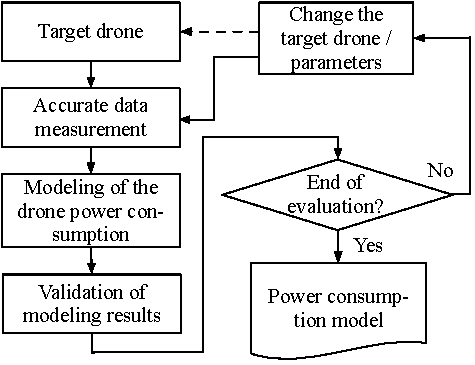
\includegraphics[scale= 0.95]{fig16/modeling_framework.pdf}}
\label{fig:freamwork_a}
\qquad

\subfloat[
Sub-problem 2: Finding the minimum energy consumption path of the drone in a given mission using the accurate power consumption mode.
]{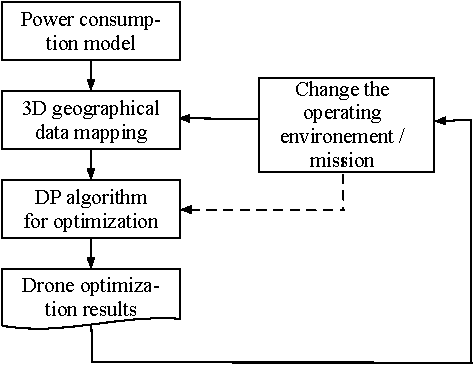
\includegraphics[scale= 0.95]{fig16/optimization_framework.pdf}}
\caption{The systematic framework of the drone optimization.}
\label{fig:freamwork_b}

\label{fig:freamwork}
\end{figure}









\section{Accurate drone power measurement}
\label{Section: Challenges in drone power measurement}





\subsection{Inaccurate data from genuine flight computer}

Top-of-the-line commercial drones provide flight data such as power consumption and GPS location during the flight. 
We use the DJI Matrice 600 Pro (M600), which is a flagship model of DJI\,\cite{ref_11}, one of the world-leading drone companies. 
M600 is equipped with an A3 flight control module that includes an onboard measurement circuit for the flight data at a sampling rate of 200 Hz. However, it turns out that the factory onboard measurement circuit is not accurate enough to build a power model. 
It goes without saying that the flight data should be accurate to build a useful power consumption model.
Therefore, we check the data from the A3 module securing the drone on the ground without turning on the propulsion using a high precision data acquisition device (NI DAQ)\,\cite{ref_12}. 

\begin{table}[ht]
\caption{An example of inaccurate data from the genuine flight module of M600 drone when it is parked as a ready state on the ground. (All motors and propellers are fully stopped.)}
\label{Table: motor_status}
\resizebox{0.485\textwidth}{!}{%
\begin{tabular}{|c|c|c|c|c|c|c|}
\hline
Motor number & Motor 1 & Motor 2 & Motor 3 & Motor 4 & Motor 5 & Motor 6 \\ \hline
Voltage (V)  & 51.3 & 51.1 & 51 & 51.5 & 51.4 & 51.1 \\ \hline
Current (A)  & -0.05 & -0.57 & -0.15 & 0.19 & 0 & 0.45 \\ \hline
Power (W)    & -2.56 & -29.12 & -7.65 & 9.78 & 0 & 22.99 \\ \hline
\end{tabular}%
}
\end{table}

The measured value in Table\,\ref{Table: motor_status} shows non-negligible negative current values that explain that there is a distinct DC offset in the power measurement circuit.
In order to check the DC offset correctly, we measure the power consumption of the drone during propulsion by tightly securing the drone on the ground while increasing the throttle.

\begin{figure}[ht]
\centering
\subfloat[The power measurement test on the ground.]{\includegraphics[scale= 0.95]{fig1/Ground_test.pdf}}
\qquad
\subfloat[Comparison of the current flow between NI DAQ and DJI onboard circuit measurement.]{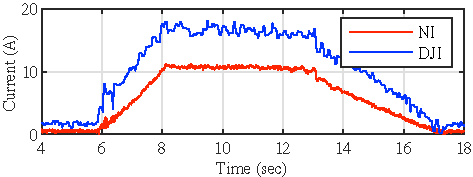
\includegraphics[scale=1.0]{fig1/NIvsDJI.pdf}}
\caption{Experiment set for the power measurement on the ground and the result.}
\label{fig:Ground_test}
\end{figure}

We configure the experiment environment for measuring the current using the shunt resistor and the operational amplifier (OP-AMP) as Fig.\,\ref{fig:Ground_test}(a) and the experiment result is presented in Fig.\,\ref{fig:Ground_test}(b). 
It visualizes that the current profile of the factory onboard power measurement circuit is marginally similar to that of the high precision data acquisition device, but the actual scale is significantly different. 
In order to overcome this difference, we attempt various trials to use the onboard power measurement circuit by post-processing (calibration, etc.). 
However, the source of error is not only the DC bias and gain error, but also sampling rate and linearity. 
We conclude that the factory onboard power measurement circuit in the drone is not appropriate for the research we aim at because of the inaccurate power data.




\subsection{Design of the power measurement board}

We design the power measurement board to exhibit a very high accuracy, like the high precision data acquisition device.
Therefore, we select parts to ensure accuracy, and we verify the measured data by comparing it with that of the same high precision data acquisition device, which is used for the evaluation of the factory onboard power measurement circuit of DJI.
We configure a power measurement board with a combination of devices and circuits, and we build a real-time operating system (RTOS) on a microcontroller unit (MCU) to schedule the operation of the MCU. 
The configured power measurement board is lightweight and separated battery-powered, so that does not affect the power consumption of the drone.

\begin{figure}[ht]
\centering
\subfloat[The front of the circuit board.]{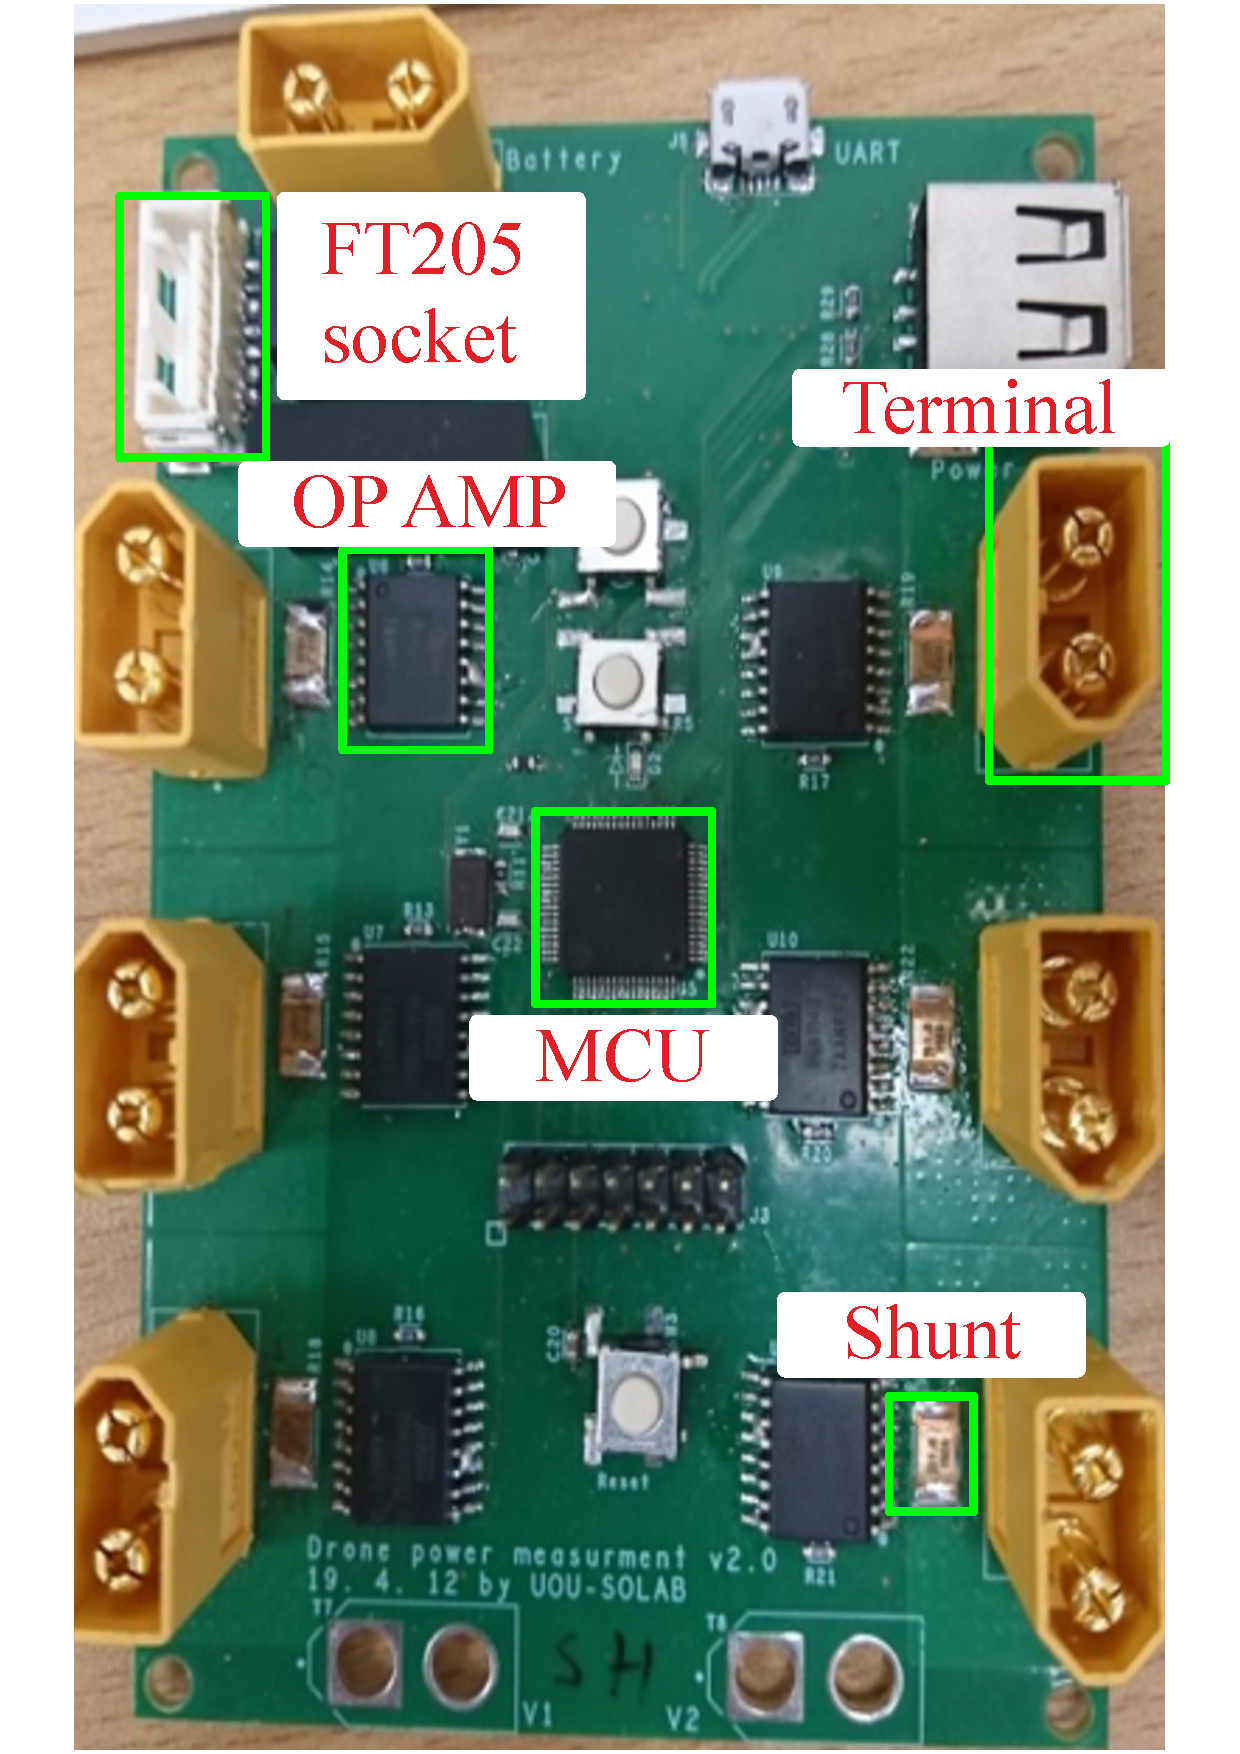
\includegraphics[scale=0.21]{fig2/New_board_front.pdf}}
\subfloat[The back of the circuit board.]{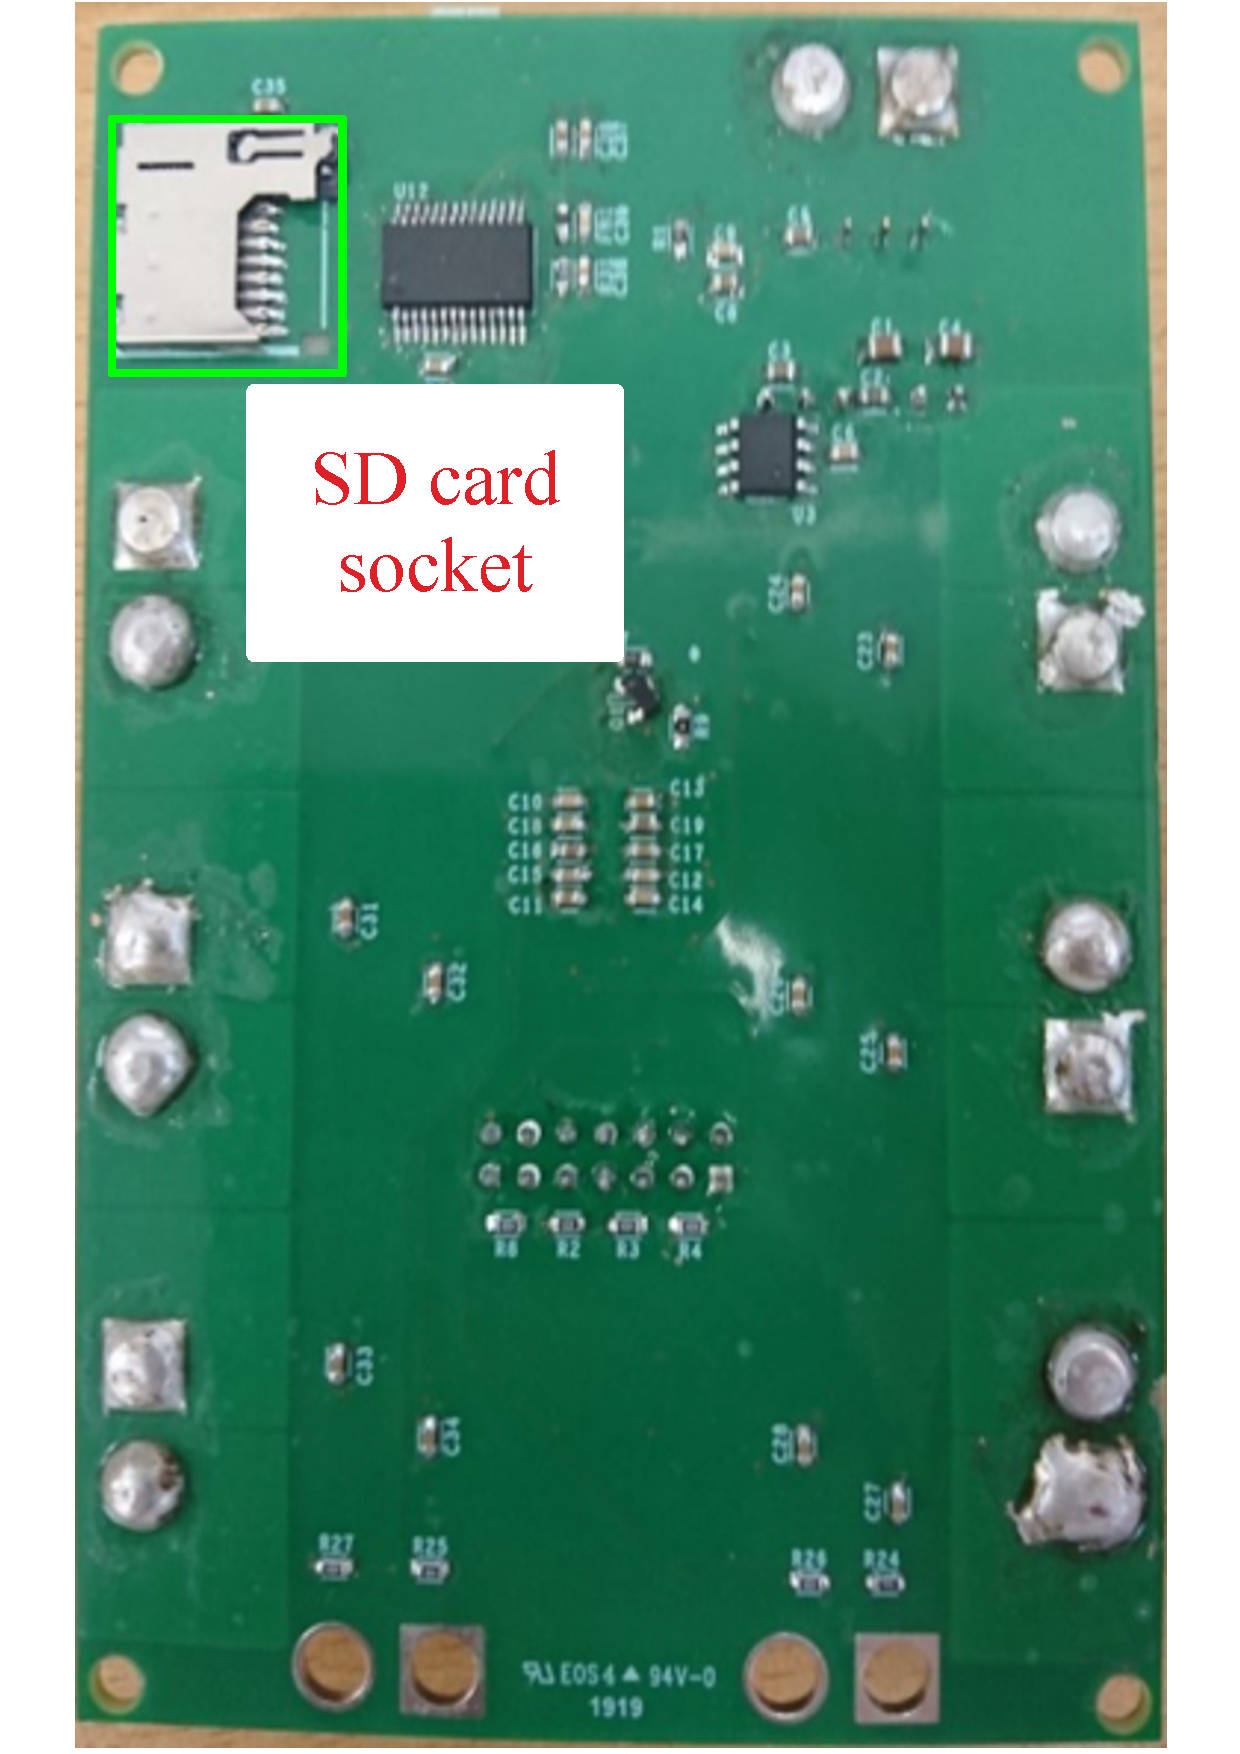
\includegraphics[scale=0.21]{fig2/New_board_back.pdf}}
\caption{The power measurement board installed on the drone.}
\label{fig:board}
\end{figure}

The power measurement board acquires the battery voltage using a voltage divider circuit under an upper limit of 52\,V, the voltage at which the M600 operates. 
The power measurement board also acquires the current of the drone using a 1\,milliohm shunt resistor and an amplifier.
The values of measured voltage and current are stored to the SD card as the binary format file that is readily processed externally.
All measurement tasks store data at a sampling rate of 1\,kHz under the management of FreeRTOS real-time operating system.
The completed board is shown in Fig.\,\ref{fig:board}.
How we measure the power consumption of the drone during the flight in Fig.\,\ref{fig:flight_test} and the power consumption comparison result is shown in Fig\,\ref{fig:flight_result}.
The measured current value on the power measurement board has an error of less than 6\,\% compared with the measured value with NI DAQ. 
By installing a lightweight power measurement board with high accuracy on the drone, we collect power data instead of the factory onboard power measurement circuit.

\begin{figure}[ht]
\centering
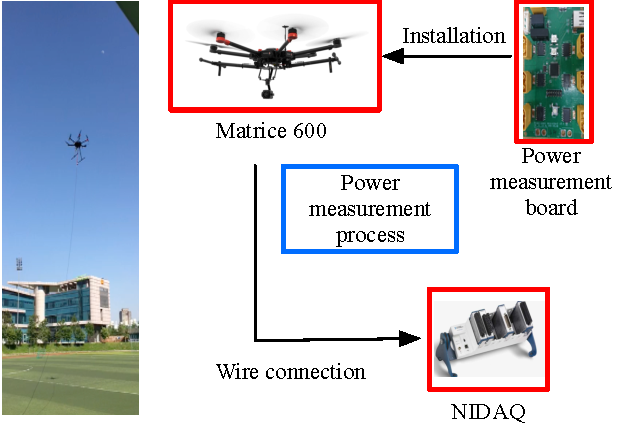
\includegraphics[scale=0.82]{fig3/flight_experiment.pdf}
\caption{The power measurement test during flight.}
\label{fig:flight_test}
\end{figure}

\begin{figure}[ht]
\centering
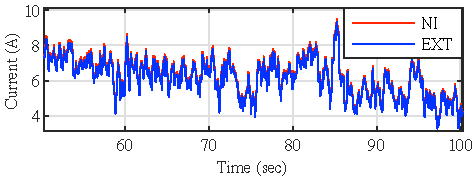
\includegraphics[scale=1.0]{fig4/flight_exp_result.pdf}
\caption{Comparison of the current measurement by each measurement device. The power measurement board presents data as accurate as NI DAQ.}
\label{fig:flight_result}
\end{figure}

\label{Section: Design the power measurement board}





\subsection{RTK GNSS}

The commercial drones always record their physical parameters such as velocity, acceleration to the backlog to confirm their flight status. 
In order to acquire parameters for use as variables in the power consumption model, we synchronize the A3 controller that is onboard genuine flight controller in M600 and our lightweight power measurement board together. 
In general, drones determine their position through the inertial measurement unit (IMU) and GPS modules. 
However, the factory onboard GPS module on M600 has a vertical error of 0.5\,m and a horizontal error of 1.5\,m, respectively. 
Such an amount of positional errors reduce power model accuracy.
Real-time kinetic (RTK) assistance GNSS is developed for enhancing the accuracy of commercial GPS.
Under the assistance of ground GPS station, RTK GNSS enhances the GPS accuracy to reduce the error to the order of cm\,\cite{ref_13}.
We install RTK GNSS on the drone and validate the improved accuracy by comparing it with another separate industrial high precision GPS module ATK980R\,\cite{ref_14}.
We conduct the following simple experiment for checking the performance of GPS improved by RTK GNSS.
First, we collocate the antenna of ATK980R and the drone in the same positions. 
Then we shift both ATK980R and the drone by a specific distance and compare the actual distance with GPS coordinates from the ATK980R and RTK GNSS module of the drone.
As a result of the experiment, we verify that the RTK GNSS on the drone has less than 5 cm error in any case compared with the industrial GPS module. This error is about 20 times lower than the error of the drone onboard GPS module.




\subsection{Wind sensor}

On the other hand, the wind profoundly affects the power consumption of drones as well as the other parameters such as velocity, acceleration.
For example, if a drone flies in the same direction as the wind, the drone consumes less power; if the drone flies in the opposite direction as the wind, the power consumption increases as the air resistance increases. 
This phenomenon becomes more severe if the overall surface area of the drone increases.
Therefore, it must be necessary to take account of the wind effect as a factor in the power consumption model of drones. 
However, measuring wind speed and direction in real-time is very difficult because turbulence frequently occurs at high altitudes in which the drone flies, and the effects of air irregularities on the drone are unpredictable.
Many studies conduct experiments using artificial wind or wind information of the region where the drone is flying provided by the national meteorological agency\,\cite{ref_5,ref_9}. 
Nevertheless, it is true that in the real situation, the drone encounters the turbulence that changes the drone's altitude or velocity; 
In this work, we measure the actual wind that affects the power consumption of drones. 
We attach the wind sensor FT205\,\cite{ref_15} in Fig.\,\ref{fig:wind_sensor} on the drone. 

\begin{figure}[ht]
\centering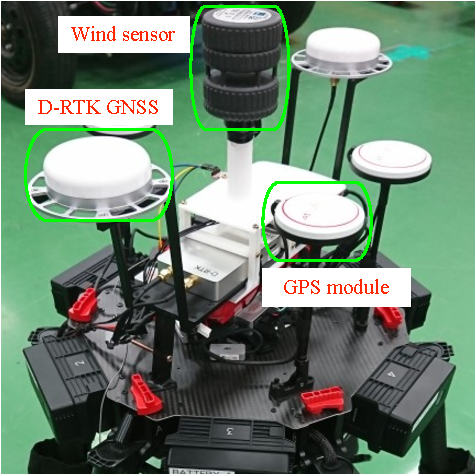
\includegraphics[scale=0.95]{fig5/wind_sensor.pdf}
\caption{The picture of installed DJI's RTK GNSS and external wind sensor FT-205.}
\label{fig:wind_sensor}
\end{figure}

The wind sensor measures the direction and speed of the wind affecting the drone with a sampling rate of 10\,Hz and a maximum error of 0.3\,m/s.
The wind data measured by the wind sensor is also stored in the SD card of the power measurement board with the power consumption data of the drone.




\subsection{Weight and volume of payload}

As the total weight of a drone increases, the thrust demanded by the drone to perform the flight increases, increasing the power consumption of the drone. 
Also, when a drone delivers a payload, the wind resistance increases by the surface area of the shipment, which also affects power consumption.
In order to confirm the impact of weight and surface area on the power consumption of M600, we collect data by varying the shape of boxes and the weight of payloads and then include the data to the power consumption model.
However, too heavy loads are very inefficient to be transported by drones, so the experiment was carried out by adding up to 2\,kg, which is about half the weight that M600 can carry.

\begin{figure}[ht]
\centering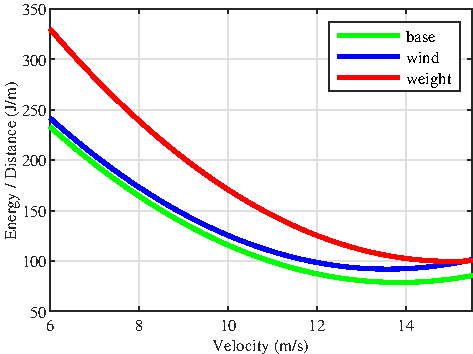
\includegraphics[scale=1.0]{fig10/t_lift.pdf}
\caption{The effect of the translational lift on the optimal velocity for the least energy consumption per meter.}
\label{fig: lift}
\end{figure}

We identify the optimum energy velocity of the drone inferred by the Helicopter effective translational lift for confirming the changes in the power consumption of the drone, as shown in Fig.\,\ref{fig: lift}.
Helicopter effective translational lift, commonly called translational lift in aerodynamics, always occurs when the rotor blades move horizontally. 
When a rotor-craft moves at a certain velocity, no vortices occur in the rotor-craft, and the air flows horizontally, then the lift force increases due to the airflow decreasing the induced drag of the drone. 
This additional lift at a certain velocity is called the effective translational lift, and this characteristic is affected by the features of the drone (weight, surface area, etc.). 
The translational lift should be used when operating the drone at the maximum performance\,\cite{ref_20}.
Based on the collected data, we present the velocity range in which the M600 can efficiently utilize energy under the effect of the translational lift. 
The green line in Fig.\,\ref{fig: lift} is the energy consumed per distance versus the constant velocity of the drone without any payload when the wind sensor records the weak wind speed between 0\,m/s to 1\,m/s that the wind does not affect the power consumption of the drone.
The red line is the energy consumed per distance versus the constant velocity of the drone with the payload of 2\,kg when the wind sensor records the weak wind speed between 0\,m/s to 1\,m/s.
The blue line is the energy consumed per distance versus the constant velocity of the drone without the payload when the wind sensor records the wind speed between 6\,m/s to 8\,m/s that the wind strongly affects the power consumption of the drone.

When an overall surface is increased, the drag force received by the drone increases, increasing the total power consumption and decreasing the optimal speed slightly. 
On the other hand, when the weight is added, the total power consumption and the optimal velocity of the drone dramatically increases.
As the above results, the drone has various optimum flight velocity according to the environment, and the optimal method of operating the drone can be determined by combining the optimum flight velocity and the battery consumption of the drone.
Note that when the weight is added to the drone, the velocity based on the translational lift exceeds the M600's safe operating range (up to 18 m/s without the wind). Unavoidably, we cannot experiment in this paper to determine the effect of payload weights because of a safety issue. 









\section{Building power consumption model of drones}
\label{Section: Power consumption model for drones}
As we mentioned in Section\,\ref{Section: Related works}, power consumption models of drones can be classified into the aerodynamics based modeling, the motor power based modeling, or the data-based modeling. 
We use the deep neural networks, one of the techniques of machine learning, to build a model based on the power consumption data and other measurable parameters that affect the power consumption of the drone collected in Section\,\ref{Section: Challenges in drone power measurement}.
The model is constructed using simple parameters that can represent the motion of the drone instead of the theory-based formulas as in the conventional regression method. 
Besides, since neural networks can theoretically approximate all functions, it is possible to predict the complex power consumption process of drones well.
In this section, we present the grid search results that are the optimal structure of the neural networks to construct an optimized model. 
We also verify the power consumption model and show the accuracy of the model on the four kinds of benchmark flights.





\subsection{Deep Neural Network}

%The Deep Neural Network (DNN) is the technique that automatically constructs the model as the form of a black box by complex mathematical equations when data is input.
%The algorithm can predict and classify a target based on the attributes learned through training data. 
%DNNs consist of several hidden layers between the input layer and the output layer.
%As the hidden layers become deeper, the characteristics of the input data can be more abstracted through each hidden layer.
%DNNs can extract characteristics from input data and create a complex model with few data elements, unlike the conventional data regression methods.
%However, DNNs have a disadvantage in that the complex relationship between the input set and the neural net structure is unknown since it is based on a black box model. 
%Therefore, there is no clear criterion on how to select the hyper-parameters such as learning rate, hidden layers, and the number of neurons to construct the optimal structure of the DNNs. 
%When constructing a model for the power consumption prediction using DNNs, the hyper-parameters of DNNs should be set optimally to increase the accuracy of the model and prevent over-fitting between the model and training data to minimize the adverse effects on the model.
%In order to find optimized hyper-parameters of DNNs, users should repeat the sequence searching the hyper-parameters of DNNs. 
The most frequently used methods of optimizing the hyper-parameters of DNNs are the random search method and the grid search method\,\cite{ref_16}. 
Between them, we use the grid search method that obtains the best result in a given space, and then we record the performance metric as Root Mean Squared Error Percentage (RMSEP) for each hyper-parameter combination.
We search the number of hidden layers from 3 to 70 and the number of hidden neurons from 10 to 100. 
The learning rate is progressed by decaying the learning rate function in the TensorFlow from 0.01, and the batch size is gradually increased by a power of 2 from 64 to 4096.
We use both the Rectified Linear Unit (ReLU) and the linear function as activation functions for the hidden layers and the output layer, respectively. 
Also, we use ADAM and SGD algorithm are used as a candidate for the learning algorithms\,\cite{ref_17}. 
The input variables of DNNs are three-axis velocity and acceleration, altitude, the total weight of the drone, two-axis wind velocity, and surface area of loads. 
We train the DNNs with 30 hours of data. Randomly excluded 0.5\,\% of the total data remains for the validation of the trained model.
The grid search is performed for 370 hours on the system consists of Intel\textregistered \,i7-8086K CPU @ 4.00\,GHz (12 cores) and NVIDIA\textregistered \,GeForce 1080Ti 16\,GB.
After recording the measured performance for each hyper-parameter set (combination), we select the hyper-parameter set (combination) that performed the highest performance.
We present the Table\,\ref{Table: gridsearch_result} that the top 7 accuracy ranking list of hyper-parameter sets (combinations) of DNNs.
We use the model with the hyper-parameter set that has the lowest error rate as the power consumption model. 
As a result, our power consumption model has the learning rate of 0.0005, 44 neurons, 35 hidden layers, 2048 batch size, ReLU for the activation function, and ADAM for the learning algorithm. 

\begin{table}[ht]
\caption{The list of grid search results}
\label{Table: gridsearch_result}
\resizebox{0.485\textwidth}{!}{%
\begin{tabular}{|c|c|c|c|c|c|l|}
\hline
Epoch & Learning late & Neurons & Hidden layers & Batch size & Optimizer & {RMSEP} \\ \hline
690   & 0.0005  & 44 & 35 & 2048 & ADAM & 8.37526 \\ \hline
494   & 0.001   & 60 & 60 & 2048 & ADAM & 8.40487 \\ \hline
277   & 0.0003  & 80 & 60 & 2048 & ADAM & 8.42413 \\ \hline
794   & 0.0002  & 44 & 35 & 4096 & ADAM & 8.45175 \\ \hline
709   & 0.001   & 44 & 30 & 512  & ADAM & 8.46091 \\ \hline
844   & 0.005   & 36 & 25 & 4096 & ADAM & 8.51061 \\ \hline
577   & 0.0005  & 36 & 35 & 512  & ADAM & 8.52163 \\ \hline
\end{tabular}%
}
\end{table}

\label{Section: Deep Neural networks (DNN)}


\subsection{Validation of power consumption model}

We configure the environment of the drone flight for verifying our power consumption model. 
The onboard SDK provided by DJI is used in conjunction with the meta software Robot Operating System (ROS), which is often used in the robotics field, to simulate the automatic driving of drones. 
Autonomous driving simulation of the drone through the program is much easier to adjust the velocity and acceleration required for the drone operation than the direct control by the user.
In order to validate the accuracy of the power consumption model, we upload the autonomous driving simulation program to the drone to perform the actual flight and compare the power consumption predicted by the power consumption model with the real power consumption. 
The onboard SDK environment of M600 for autonomous driving simulation is shown in Fig.\,\ref{fig:SDK}.

\begin{figure}[h]
\centering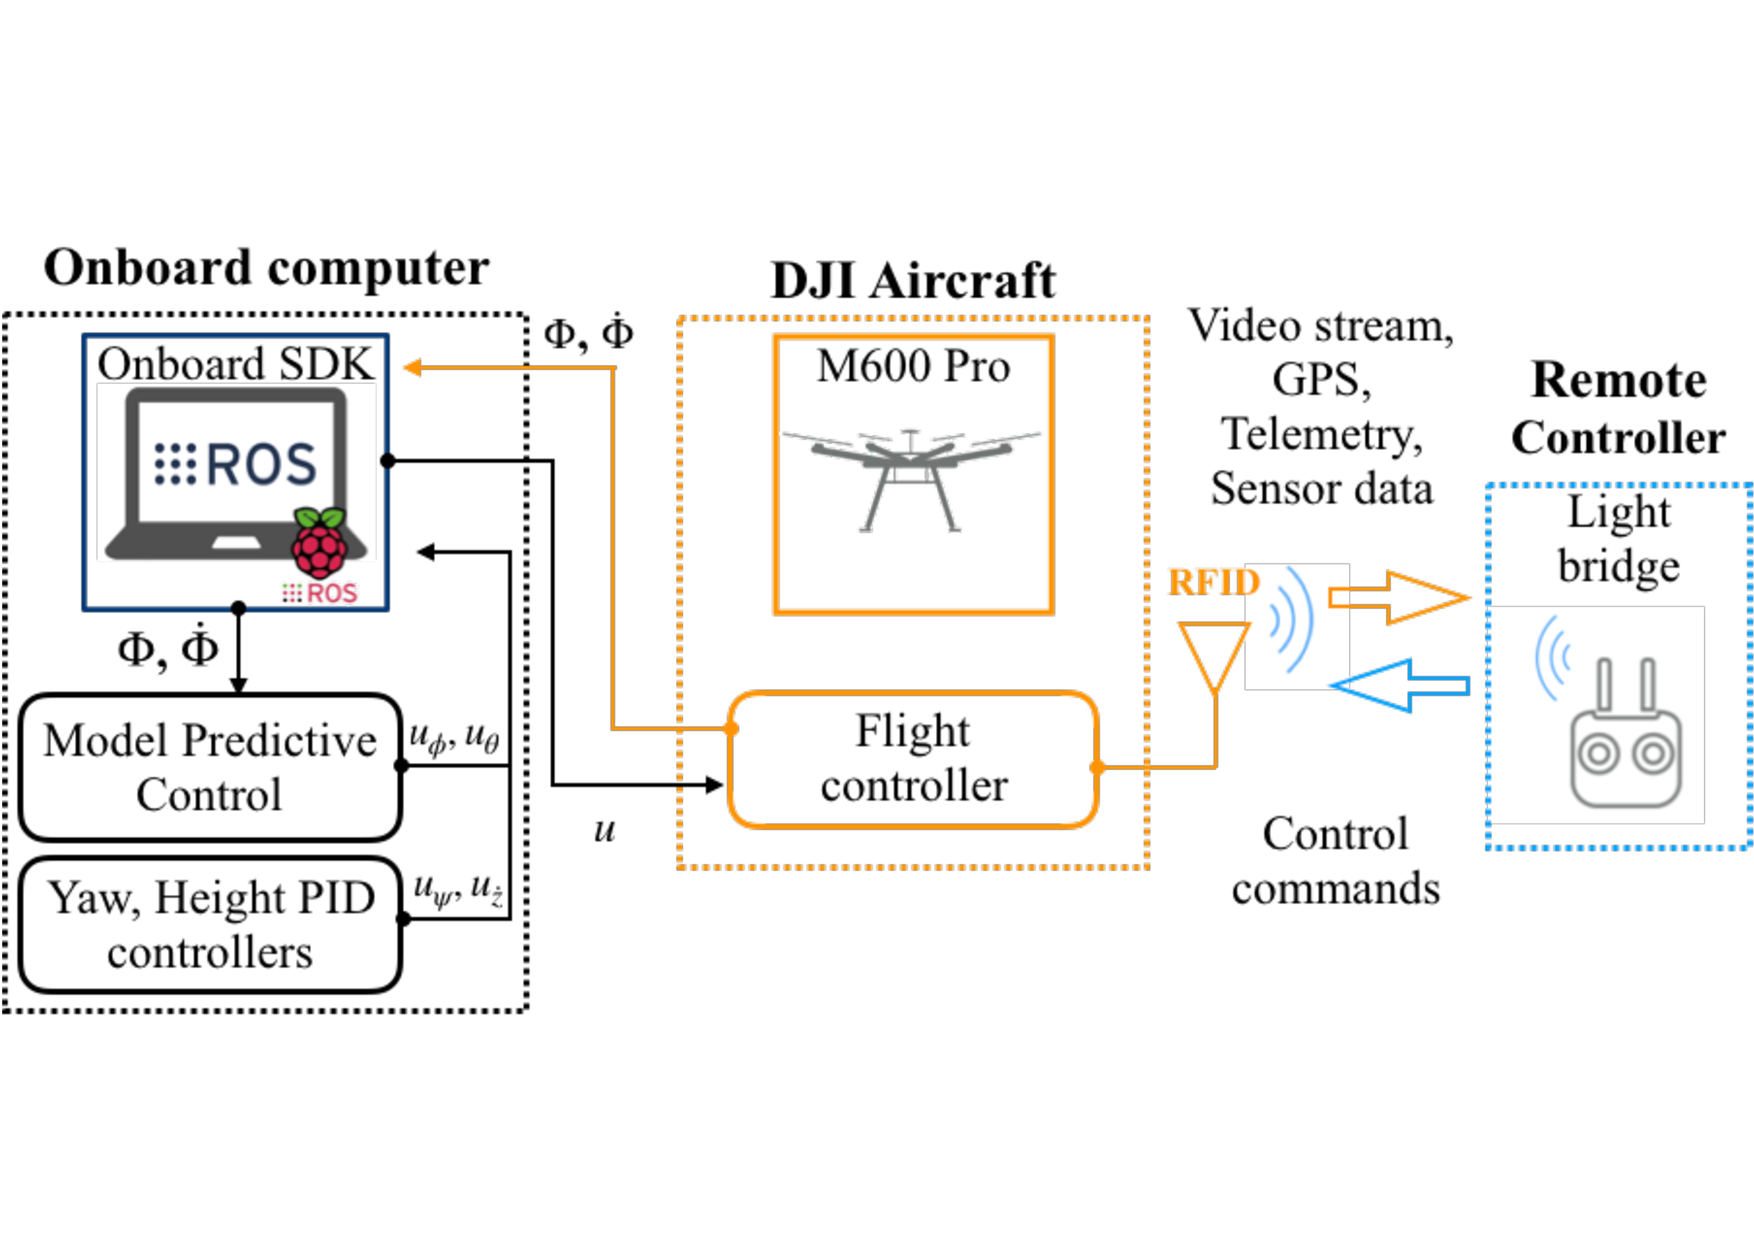
\includegraphics[scale=0.285]{fig7/SDK.pdf}
\caption{The onboard SDK system for automatic flight of drones}
\label{fig:SDK}
\end{figure}

\begin{figure}[h]
\centering
\subfloat[Drone power consumption when hovering.]{\centering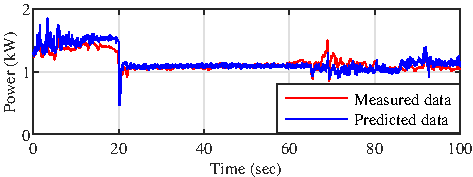
\includegraphics[scale=1.05]{fig8/Hover8x3.pdf}}
\qquad
\subfloat[Drone power consumption when ascending and descending.]{\centering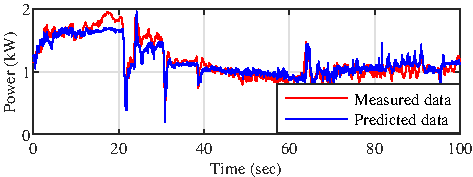
\includegraphics[scale=1.05]{fig8/AD8x3.pdf}}
\qquad
\subfloat[Drone power consumption when interval flight.]{\centering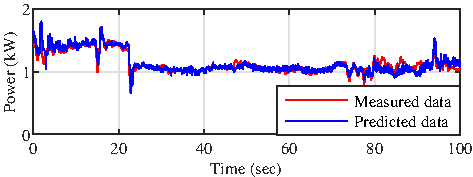
\includegraphics[scale=1.05]{fig8/Interval8x3.pdf}}
\qquad
\subfloat[Drone power consumption when squared-shaped flight.]{\centering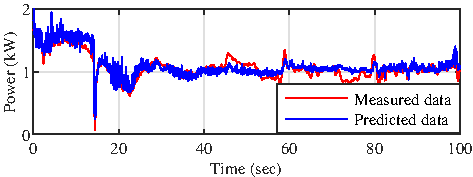
\includegraphics[scale=1.05]{fig8/Square8x3.pdf}}
\qquad 
\subfloat[Comparison result of the power consumption model with payload and without payload during constant speed flight of 6\,m/s.]{\centering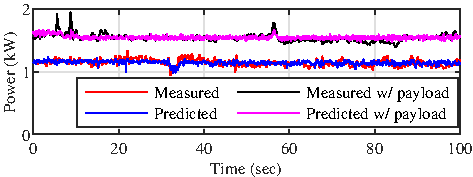
\includegraphics[scale=1.05]{fig9/compare_weight8x3.pdf}}

\caption{Comparison of measured power consumption and predicted power consumption under the benchmark flights.}

\label{fig: benchmark}
\end{figure}

When comparing the power after the actual flight with a drone, Fig.\,\ref{fig: benchmark} shows the measured power and estimated power when i) the drone is hovering in the air, ii) the drone repeats vertical flights (ascending and descending without horizontal movement), iii) the drone is flying an interval flight path that repeats horizontal flights (straight flight and back straight flight without vertical movement), and iv) the drone is flying a rectangular and level flight path, respectively. 
We compare the power estimated by the proposed power model with the measured flight data and confirm that the error of each benchmark test is 6.27\,\%, 9.8\,\%, 7.82\,\%, and 9.12\,\%, respectively.


\begin{comment}
\subsection{Effect of weight and surface area on drones}
As mentioned earlier, it is very important to consider the weight of the drone and the effects of wind when referring to drone such as drones.
As the total weight of a drone increases, the thrust demanded by the drone to perform the flight increases, increasing the power consumption of the drone. 
Also, when a drone delivers a payload, the wind resistance increases by the surface area of the shipment, which also affects power consumption.
We collect data by varying the shape of boxes and the weight of payloads and then include the collected data in the training data of the power consumption model.
However, too heavy loads are very inefficient to be transported by drones, so the experiment was carried out by adding up to 2\,kg, which is about half the weight that M600 can carry.
The result of estimating the power consumed by M600 with the payload during a constant speed flight and the power consumed by a drone without payload in the same flight condition is shown in Fig.\,\ref{fig: Model_weight}. 
When comparing the results, the drone with payload consumes about 30\,\% more power, which means  the same rate also reduces the run-time of the drone.

\begin{figure}[ht]
\centering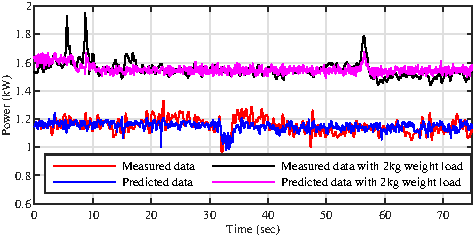
\includegraphics[scale=1.0]{fig9/compare_weight8x4.pdf}
\caption{Comparison result of the power consumption model with payload and without payload during constant speed flight of 6\,m/s.}
\label{fig: Model_weight}
\end{figure}

In order to confirm the changes in the power consumption of the drone due to the increase in the surface area, we identify the optimum energy velocity of the drone inferred by the Helicopter effective translational lift.
Helicopter effective translational lift, commonly called translational lift in aerodynamics, always occurs when the rotor blades move horizontally. 
When a rotor-craft moves at a certain velocity, no vortices occur in the rotor-craft, and the air flows horizontally, then the lift force increases due to the airflow decreasing the induced drag of the drone. 
This additional lift at a certain velocity is called the effective translational lift, and this characteristic is affected by the drone's characteristics (weight, surface area, etc.). 
The translational lift should be used when operating the drone at the maximum performance\,\cite{ref_20}.
Based on the collected data, we present the velocity range in which the M600 can efficiently utilize energy under the effect of the translational lift. 
As shown in Fig.\,\ref{fig: lift}, the energy consumption within the speed range is changed when an external influence is applied to the drone.
The green line in Fig.\,\ref{fig: lift} is the energy consumed per distance versus the constant velocity of the drone without any payload when the wind sensor records the weak wind speed between 0\,m/s to 1\,m/s that the wind does not affect the power consumption of the drone.
The red line is the energy consumed per distance versus the constant velocity of the drone with the payload of 2\,kg when the wind sensor records the weak wind speed between 0\,m/s to 1\,m/s.
Unlike the two lines, the blue line is the energy consumed per distance versus the constant velocity of the drone without the payload when the wind sensor records the strong wind speed between 6\,m/s to 8\,m/s. 


\begin{figure}[ht]
\centering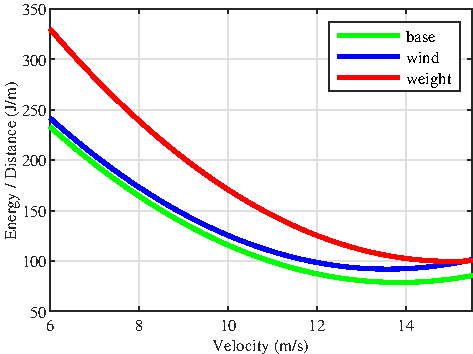
\includegraphics[scale=1.0]{fig10/t_lift.pdf}
\caption{The effect of the translational lift on the optimal velocity for the least energy consumption per meter.}
\label{fig: lift}
\end{figure}

Initially, the drone has an optimum velocity that consumes the least energy without any external attachments. 
When a box is added, in order to increase the overall surface area of the drone, the drag force received by the drone increases, increasing the overall power consumption and decreasing the optimal speed slightly. 
Adding a weight to the drone increases the overall power consumption and the optimal velocity of the drone dramatically.
As the above results, the drone has various optimum flight velocity according to the environment, and the optimal method of operating the drone can be determined by combining the optimum flight velocity and the battery consumption of the drone. 
Therefore, it is very important that the power consumption model correctly represents the fluctuations in power consumption due to the weight and wind. 
The power consumption model that can infer power consumption in any environment is the basis for optimizing the energy consumption of the drone.

Note that when the weight is added to the drone, the velocity based on the translational lift exceeds the M600's safe operating range (up to 18 m/s without the wind). Unavoidably, we cannot experiment in this paper to determine the effect of payload weights because of a safety issue. However, we will proceed with experiments using later small drones to handle heterogeneous drones.

\end{comment}






\section{Flight energy optimization}
\label{Section: Optimization}

We predict the energy consumption when a drone arrives from a starting point to a designated destination avoiding obstacles while flying downtown. 
After deriving a flight path that consumes the least energy based on the power consumption model, we validate the usefulness of our drone optimization algorithm by flying the derived route with a real drone and comparing the energy consumption.
As we mentioned in Section\,\ref{Section: Related works}, there are advantages and disadvantages in the optimization method for drones through the numerical algorithm and the graph search algorithms.
However, in order to optimize the overall operation of drones, the optimization method must consider both operating environments and operation times of the drone.
The numerical algorithms are suitable for expressing the momentary movements of the drones, but it is not ideal for calculating all the actions of the drone about half an hour at a wide range.
Therefore, we optimize the overall movement of a drone by using a graph search algorithm that can visualize the external environment of the drone.




\subsection{Configuration of optimization problem}

\begin{figure}[ht]
\centering
\subfloat[The isometric view of the visualization of the environment around which drones fly.]{\centering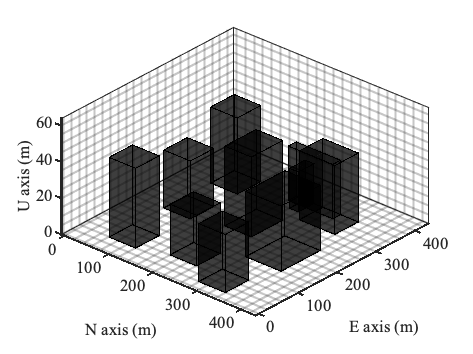
\includegraphics[scale=0.9]{fig11/obs.pdf}}
\qquad
\subfloat[The direction that the drone can move in a visualized environment.]{\centering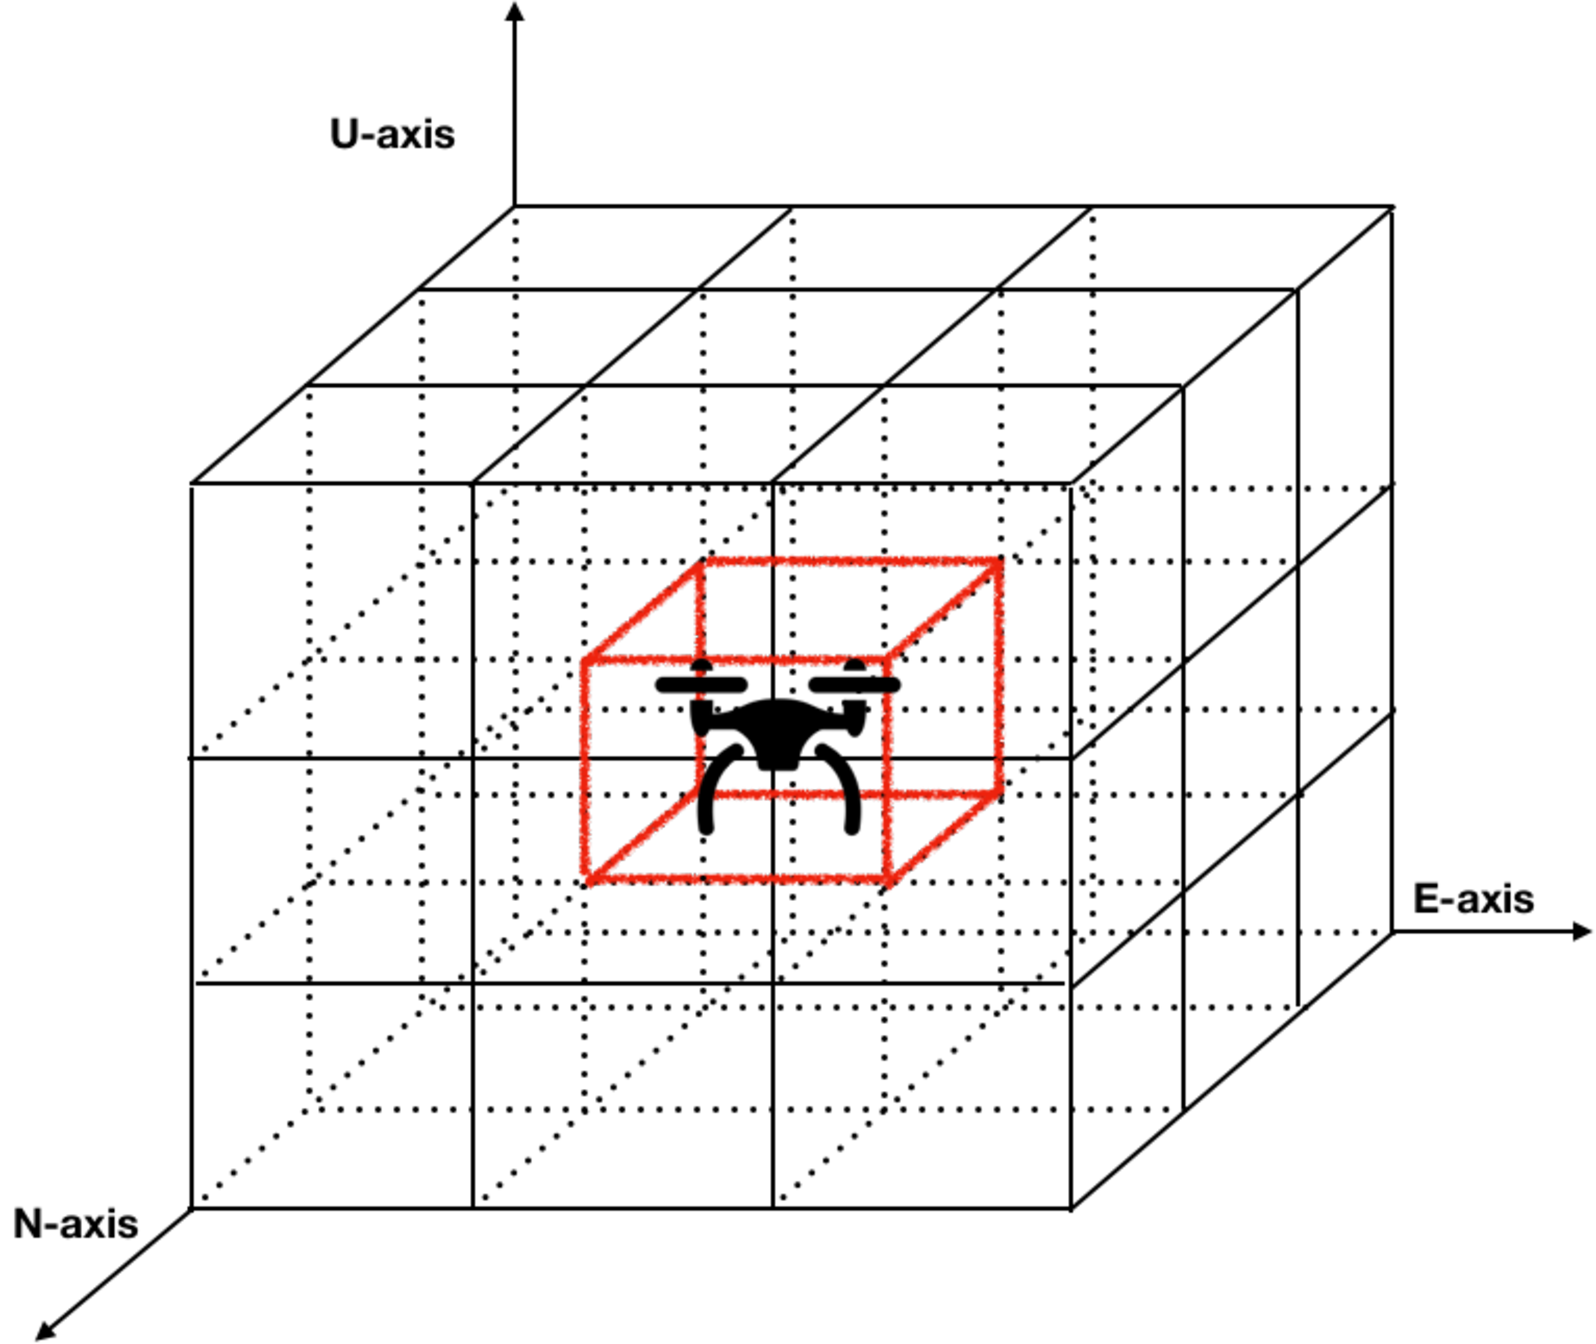
\includegraphics[scale=0.25]{fig11/Direction.pdf}}
\caption{Visualization of the drone operating environment and the drone moving direction system within the environment.}
\label{fig: opt_env}
\end{figure}

We model the operating environment of the drone as Fig.\,\ref{fig: opt_env}(a).
The environment is assumed that there are various types of building between the start and endpoints in a space where the maximum range of the N- and E-axis is 400\,m ,and the U-axis is 80\,m, respectively.
The drone in the environment can move 10\,m for each step of horizontal axis movements and 3\,m for each step of vertical axis movements, and the drone cannot pass through obstacles. 
Besides, the drone moves in one direction per step by selecting a moving direction.
In Fig.\,\ref{fig: opt_env}(b), there are 26\,directions of the drone to move from the current step to the next step.
However, when optimizing the flight path of the drone with one destination, the backward direction must be excluded because the drone consumes more energy as the operating time becomes longer. Therefore, we conclude there are a total of 17\,directions for the drone to move on to the next step.
The velocity of the drone moving between nodes is determined based on the translational lift effect in Fig.\,\ref{fig: lift} that the M600 drone consumes the least energy per distance with each case of the drone environment. 
The minimum energy consumption velocity per distance of the M600 drone can be changed at any time due to external influences.  
Previous studies using the graph search algorithm assume that objects move at a constant velocity between nodes because it is difficult to calculate the instantaneous movement of objects moving between steps\,\cite{ref_8, ref_10, ref_22}. 
On the other hand, we set the range of the drone velocity from a minimum of 6\,m/s to a maximum of 15\,m/s to explain the power consumption change by the velocity change. 
At the same time, we take into account the effect of the drone acceleration that significantly affects the drone power consumption.
We discuss the problems that arise when considering the acceleration of the drone on the optimization problem and heuristics applied to solve them in Subsection\,\ref{sub_Section: Graph search}.

Then, we construct the operating environment of drones as a graph that consists of nodes and edges from the referred three-dimensional space with the assumption that there is no influence of the radius of curvature of the earth to configure the optimization problem. 
The nodes contain the parameters of the drone and the factor of the external environment, and nodes have many edges as all the elements they contain.
The edges are paths that can be moved between the nodes and has its weight.
The edge-node graph moves between nodes by comparing the weights assigned to the edges.  
Each node of the graph contains the information in the three-dimensional space. $x_i$, $y_i$, and $z_i$ are each axis position information of the node i, and $v_i$ and $a_i$ are the velocity and acceleration of the drone at the node i. 
The velocity and direction of the wind are denoted as $w_i$ and $d_i$. The weight and surface area that increases when a load is added on the drone are constant values.
Node $n_i$ is declared as 
\begin{equation*}
n_i = (x_i, y_i, z_i, v_i, a_i, w_i, d_i).
\end{equation*}

\noindent The edges of the graph that connect between the nodes store the cost weights between the nodes.
The weights applied to each edge are the energy consumption calculated by combining the edges with the time required for the node switching and the average instantaneous power consumption of each node, which can be expressed following that: 
\begin{equation*}
E(n_j, n_k) = \frac{P(n_j)+P(n_k)}{2} \Delta t,
\end{equation*}
where $P(n_j)$ and $P(n_k)$ are the instantaneous power at the $n_j$ and $n_k$, and $\Delta t$ is the time taken to move the edge between the nodes, respectively.

The configured drone optimization problem is that the drone starts a mission at the starting point and reaches the ending point, searching for the path that consumes the least energy at each step in the graph. 
Even when an external force such as the wind effect acts on the drone, the optimization responds to the external force and derives an optimal path that consumes less energy.
We use Dijkstra's algorithm that is a dynamic programming optimization method using exhaustive search\,\cite{ref_19}. 




\subsection{Graph search algorithm to consider acceleration between each node}
\label{sub_Section: Graph search}

In contrast to the studies using the conventional graph search algorithms that use the heuristics that exclude the velocity change to reduce the dimension, we include the drone acceleration that significantly affects its power consumption. 
Therefore, we modify the graph search algorithm to consider acceleration between each unit node. 
We devise heuristics about the drone movement to solve i) how much time of the drone will accelerate between nodes and ii) how the drone between each axis of the graph can accurately reach the position of the next node when the drone proceeds to acceleration and deceleration. 
The following items are assumptions that must meet when moving between drone nodes:

\begin{itemize}
\item Heuristic 1. The distance and travel time between the current node and the next node:
  \begin{itemize}
      \item If the direction of the drone to the next node and the direction of the drone when reaching the current node are opposite, there is a difference in the travel distance when the drone decelerates and accelerates for the target velocity.
      \item The moving direction and velocity of the previous node must be stored to take into account the added travel distance and time resulting from the velocity difference between the nodes to make the drone arrive correctly at the next node.
      \item $\Delta t$ is the time that takes for one axis between nodes to reach the target node. It is set based on the axis that takes the longest time among the three axes.
      \item The velocity of the remaining axes is increased or decreased in proportion to the set $\Delta t$.
  \end{itemize}
\item Heuristic 2. The instantaneous velocity at the next node:
  \begin{itemize}
      \item The drone from the current node to the next node must reach the velocity specified in the next node by either acceleration or deceleration.
      \item The drone accelerates to the target velocity of the next node and then moves the remaining distance with uniform velocity.
      \item The acceleration of the drone uses the maximum acceleration the drone can exert, and increases linearly.  
  \end{itemize}
\end{itemize}

We regard that the drone movement must satisfy those assumptions for each axis of space, then we find $\Delta t$ that satisfies both Heuristic\,1 and\,2 for each axis is obtained through the following Algorithm\,1. 
By applying the heuristic that reaches the target node at the same time, we implement the drone optimization that can consider the acceleration of the drone in the graph search method.

\begin{algorithm}[ht]
 \caption{Finding $\Delta t$, which is the travel time between the nodes.}
 \begin{algorithmic}[1]
   \renewcommand{\algorithmicrequire}{\textbf{Input:}}
   \renewcommand{\algorithmicensure}{\textbf{Output:}}
   \REQUIRE 
   \textit {$V_c$ - The velocity of the current node} \\
   \hskip1.5em \textit{$V_n$ - The velocity of the next node} \\
   \hskip1.5em \textit{$d$ - The distance between the nodes}
   \ENSURE
   \textit{$\Delta t$ - The travel time between the nodes}
    \FOR {each axis of the graph}
    \IF {{$V_n[axis], V_c[axis] := 0$}}
    \STATE $\Delta t[axis] = \infty $
    \ELSIF {($V_n[axis] \ne 0$)}
    \STATE $\Delta t_1 := \cfrac{V_n - V_c}{2}$
    \IF {{$d[axis] = \Delta t_1 * \cfrac{\abs{V_n[axis] + V_c[axis]}}{2}$}}
    \STATE $\Delta t_2 := 0$
    \ELSE 
    \STATE $\Delta t_2 := \cfrac{(d[axis] - \Delta t_1 * \cfrac{\abs{V_n[axis] + V_c[axis]}}{2})}{\abs{V_n[axis]}}$
    \ENDIF
    \ELSE
    \STATE $\Delta t_1 := \cfrac{V_n[axis] - V_c[axis]}{2}$
    \IF {($d = \Delta t_1 * \cfrac{\abs{V_n[axis] + V_c[axis]}}{2}$)}
    \STATE $\Delta t_2 := 0$
    \ELSE 
    \STATE $\Delta t_2 := \cfrac{(d[axis] - \Delta t_1 * \cfrac{\abs{V_n[axis] + V_c[axis]}}{2})}{\abs{V_c[axis]}}$
    \ENDIF
    \ENDIF
    \STATE $\Delta t[axis] = \Delta t_1 + \Delta t_2$
    \ENDFOR
    \RETURN $\Delta t = max(\Delta t)$ 
 \end{algorithmic} 
\end{algorithm}









\section{Experimental Results}
\label{Section: results}

We present the baseline and the flight path derived through optimization in one environment to compare the difference between the optimized flight path and the flight path of a typical drone.
There is the result of the optimization for minimum energy consumption path considering Section\,\ref{Section: Power consumption model for drones}, as shown in Fig.\,\ref{fig: opt_environ}.
The optimal flight path in Fig.\,\ref{fig: opt_environ} excludes the wind effect to compare the difference in energy consumption only in the path changes.
The proposed baseline is a path that arrives at the shortest path through linear movement between the starting point and the arrival point using the waypoint function of the drone. The drone in the baseline moves up to the maximum height of the obstacle between the starting point and the ending point, then moves straight to the ending point and descends to the altitude of the ending point. 
In the case of the optimal flight path, the drone bypasses the obstacles it encounters while flying between the starting point and the ending point or moves up to the height of the obstacles to overcome them. 
The movement velocity of the drone in the two paths is based on the translational lift effect.
The baseline maintains the uniform velocity that achieves the minimum energy consumption over the distance. 
At the baseline, the total power consumption by the drone from the start point to the ending point is 49.78\,kJ.
On the other hand, the optimum path has a change in the velocity for each specific section in the path changed by the obstacle. 
The total power consumed by the proposed optimal path is 46.1\,kJ, which is 8.4\,\% more efficient than the baseline. 


\begin{figure}[ht]
\centering
\subfloat[The isometric view of the baseline and optimized path in the drone flight environment.]{\centering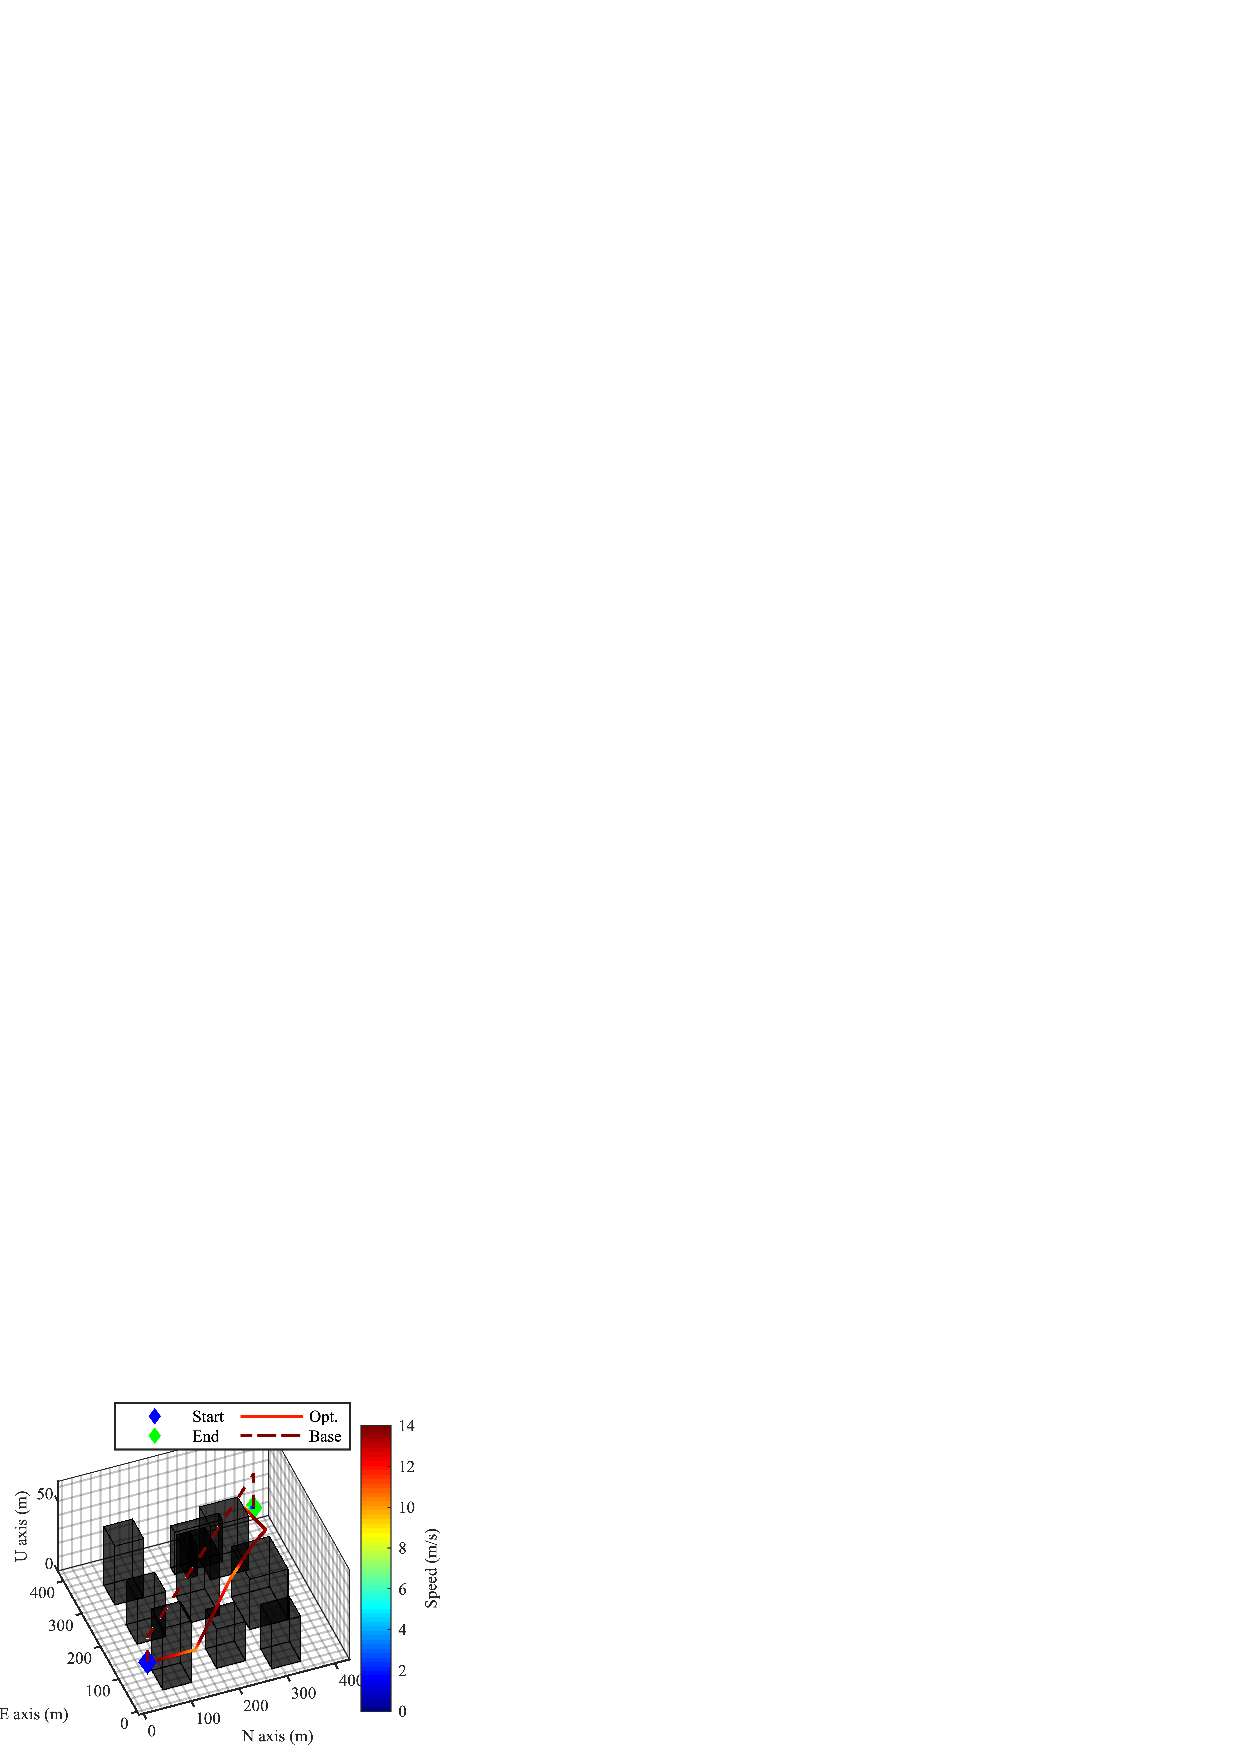
\includegraphics[scale=1.0]{fig13/opt_iso.pdf}}
\qquad
\subfloat[The top view of the baseline and optimized path in the drone flight environment.]{\centering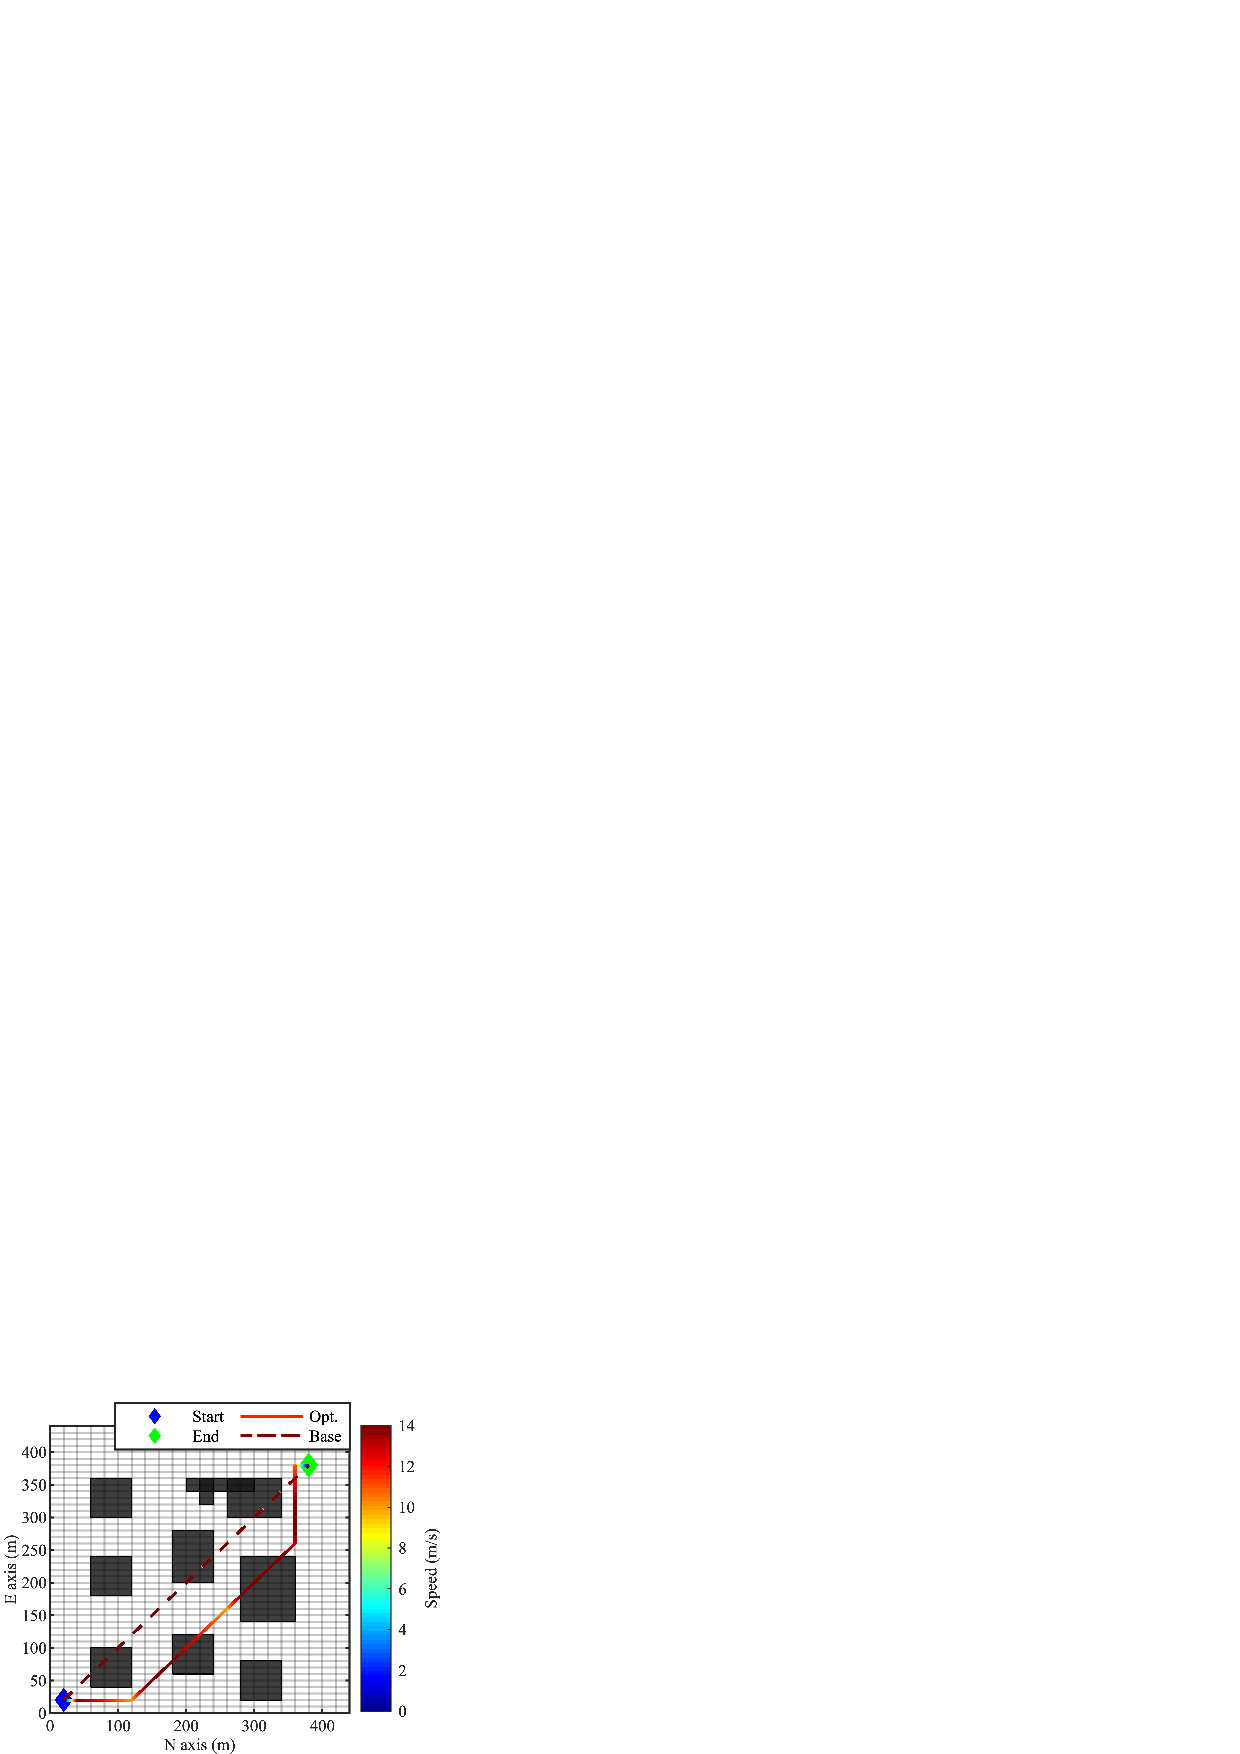
\includegraphics[scale=1.0]{fig13/opt_top.pdf}}
\caption{The energy minimum optimization result of drone in the drone flight environment.}
\label{fig: opt_environ}
\end{figure}

\begin{figure}[ht]
\centering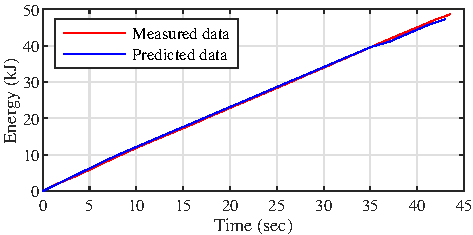
\includegraphics[scale=1.0]{fig14/S_E.pdf}
\caption{Comparison of the total energy consumption value by the simulator calculation and M600 flight measurement through the travel distance.}
\label{fig:consumed_energy}
\end{figure}

The optimal path saves energy by avoiding a sudden increase in motor output, such as bypassing a high-level obstacle or overcoming a low-level obstacle in a nearby environment instead of overcoming the highest obstacle in the path.

\begin{figure*}[htp!b]
\centering
\subfloat[The case 1 of the energy minimum path optimization of the drone affected by wind effect.]{\centering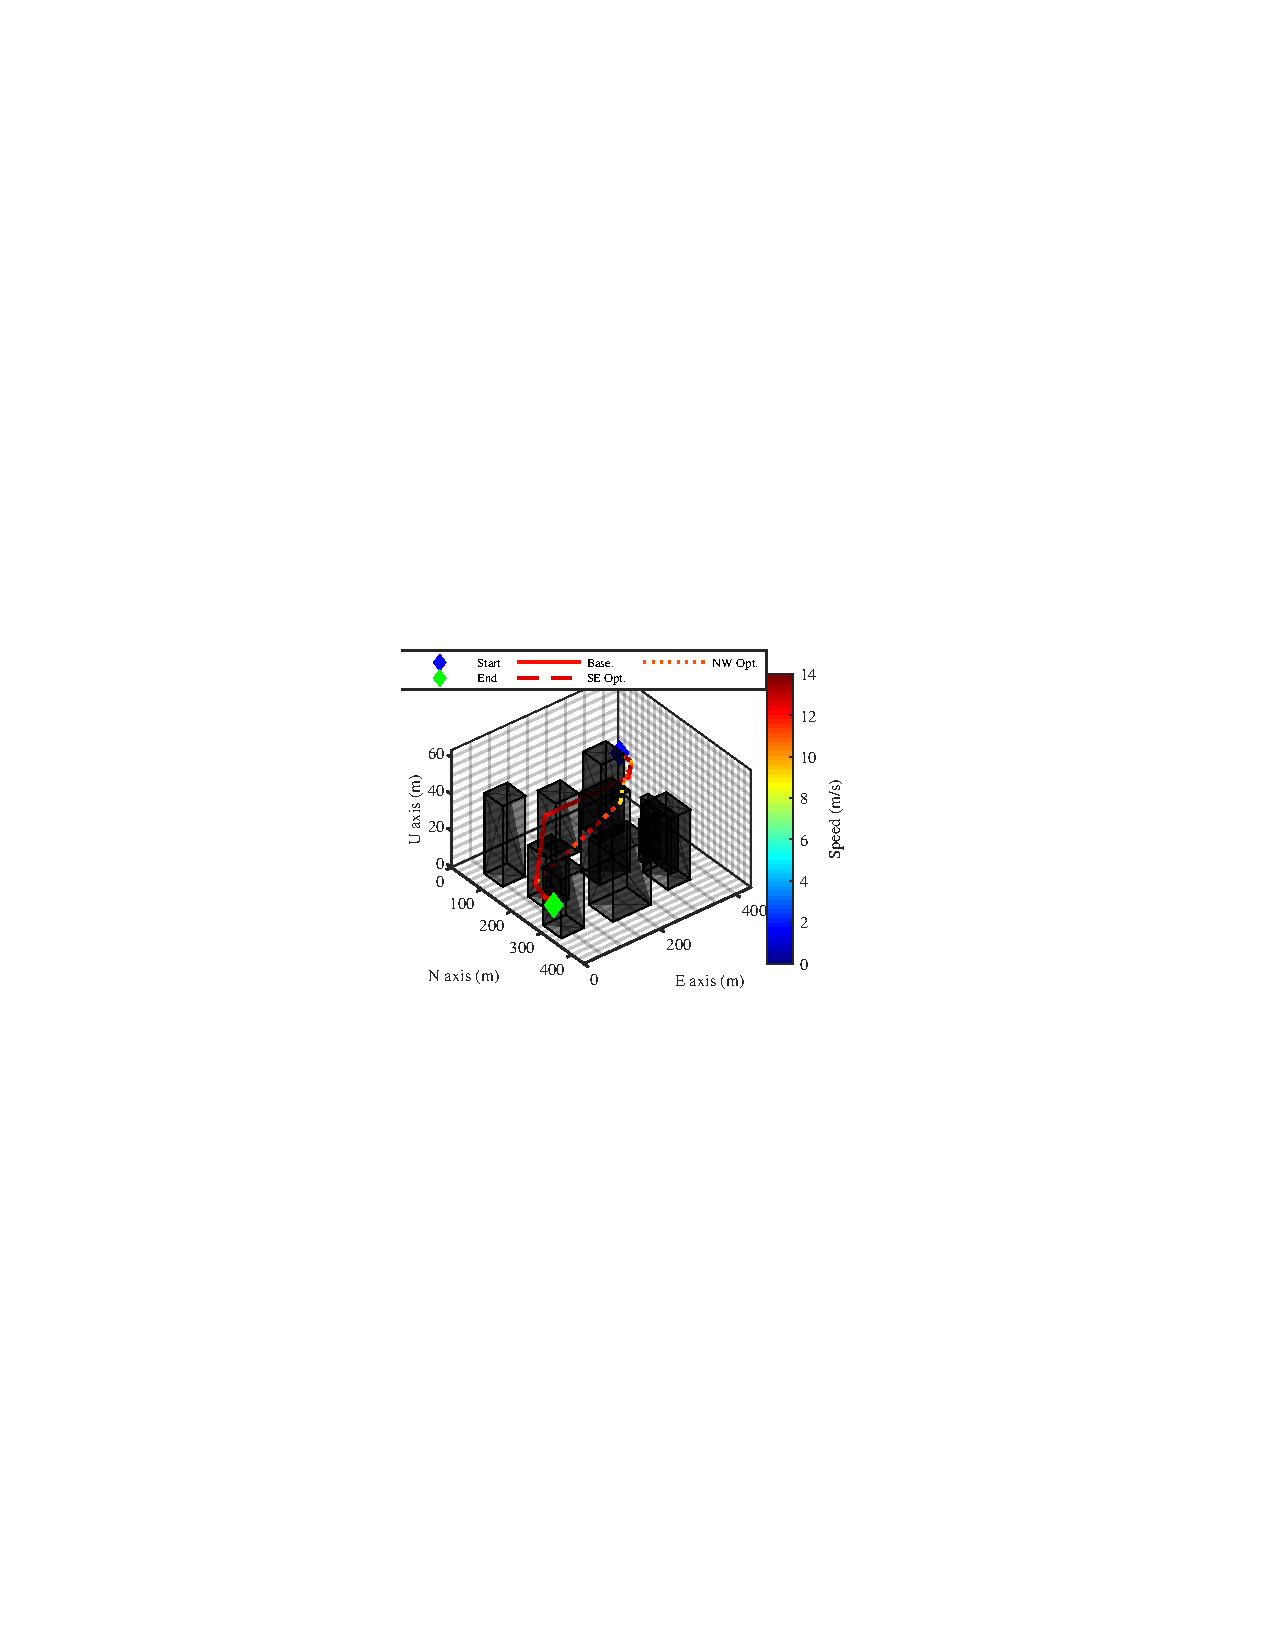
\includegraphics[scale=0.71]{fig15/case1.pdf}}
\subfloat[The top view of case 1.]{\centering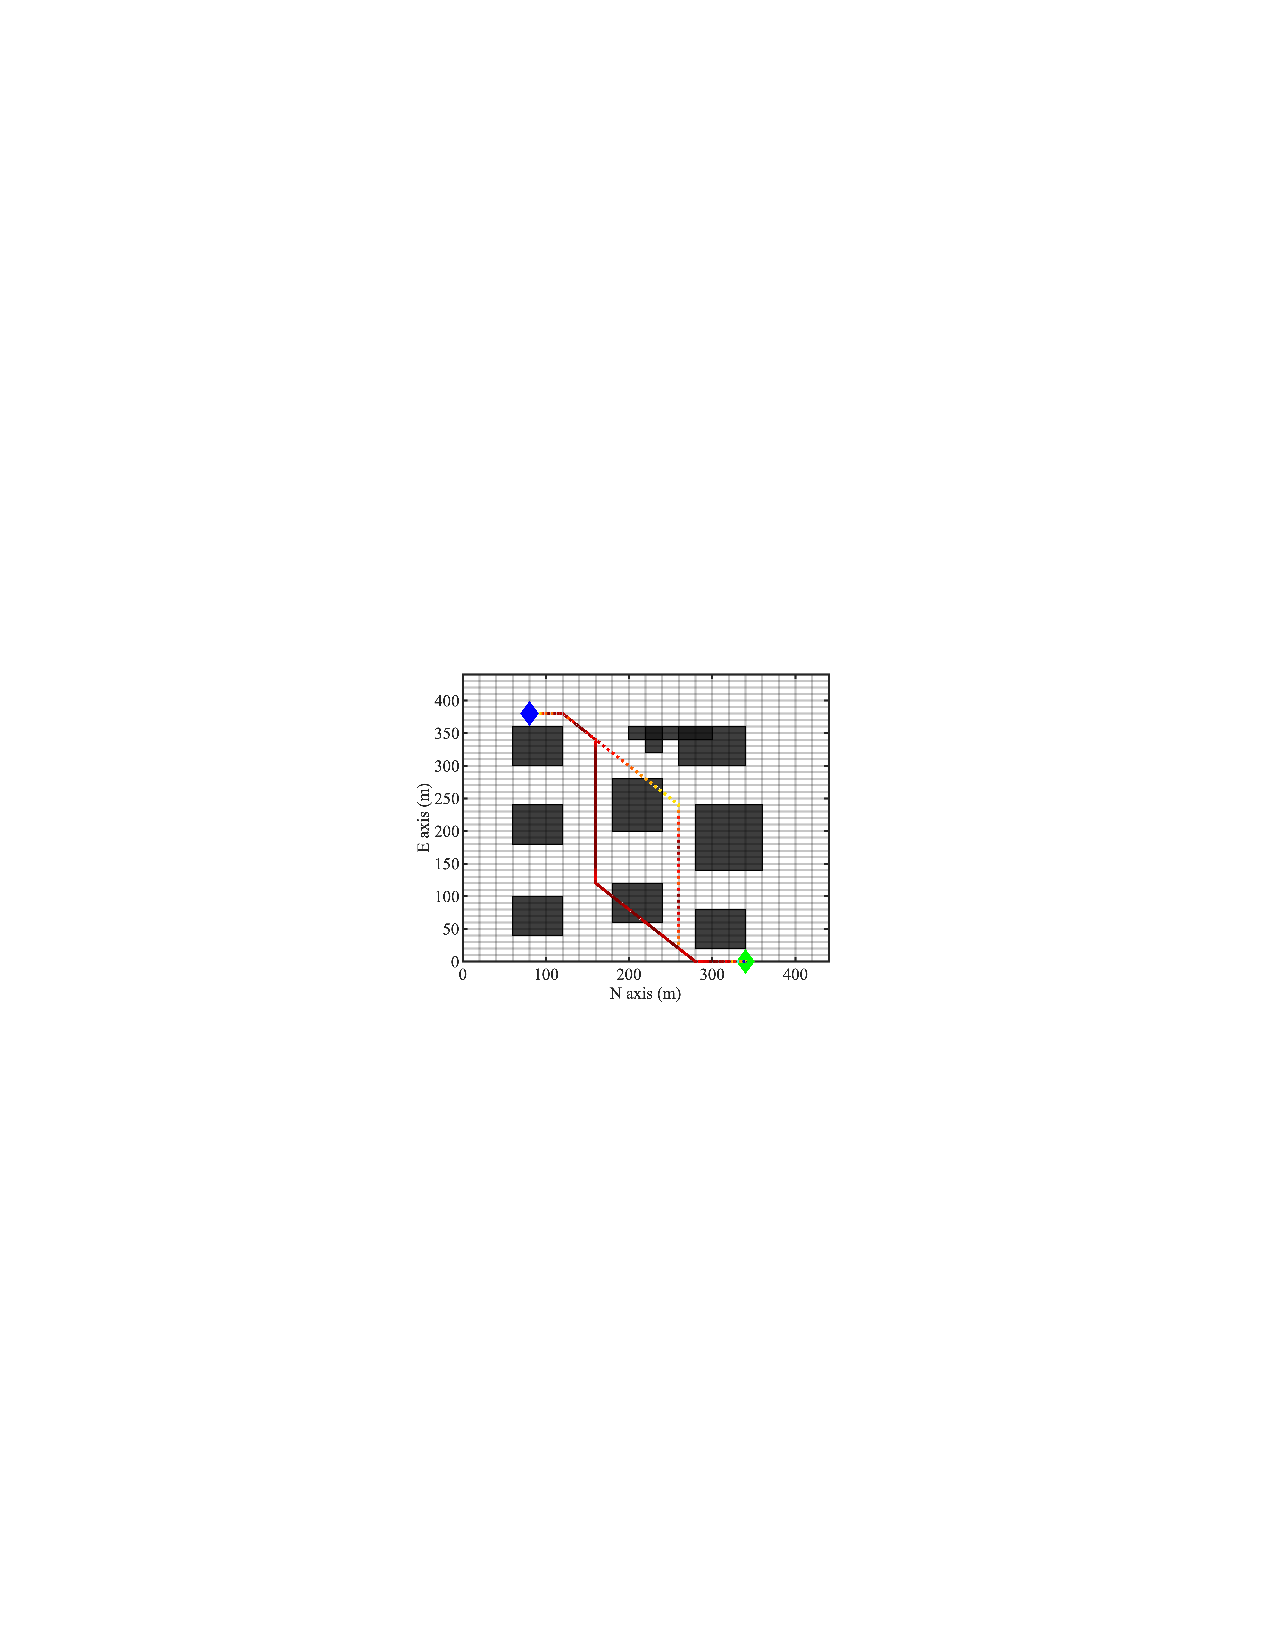
\includegraphics[scale=0.71]{fig15/case1_top.pdf}}
\subfloat[The side view of case 1.]{\centering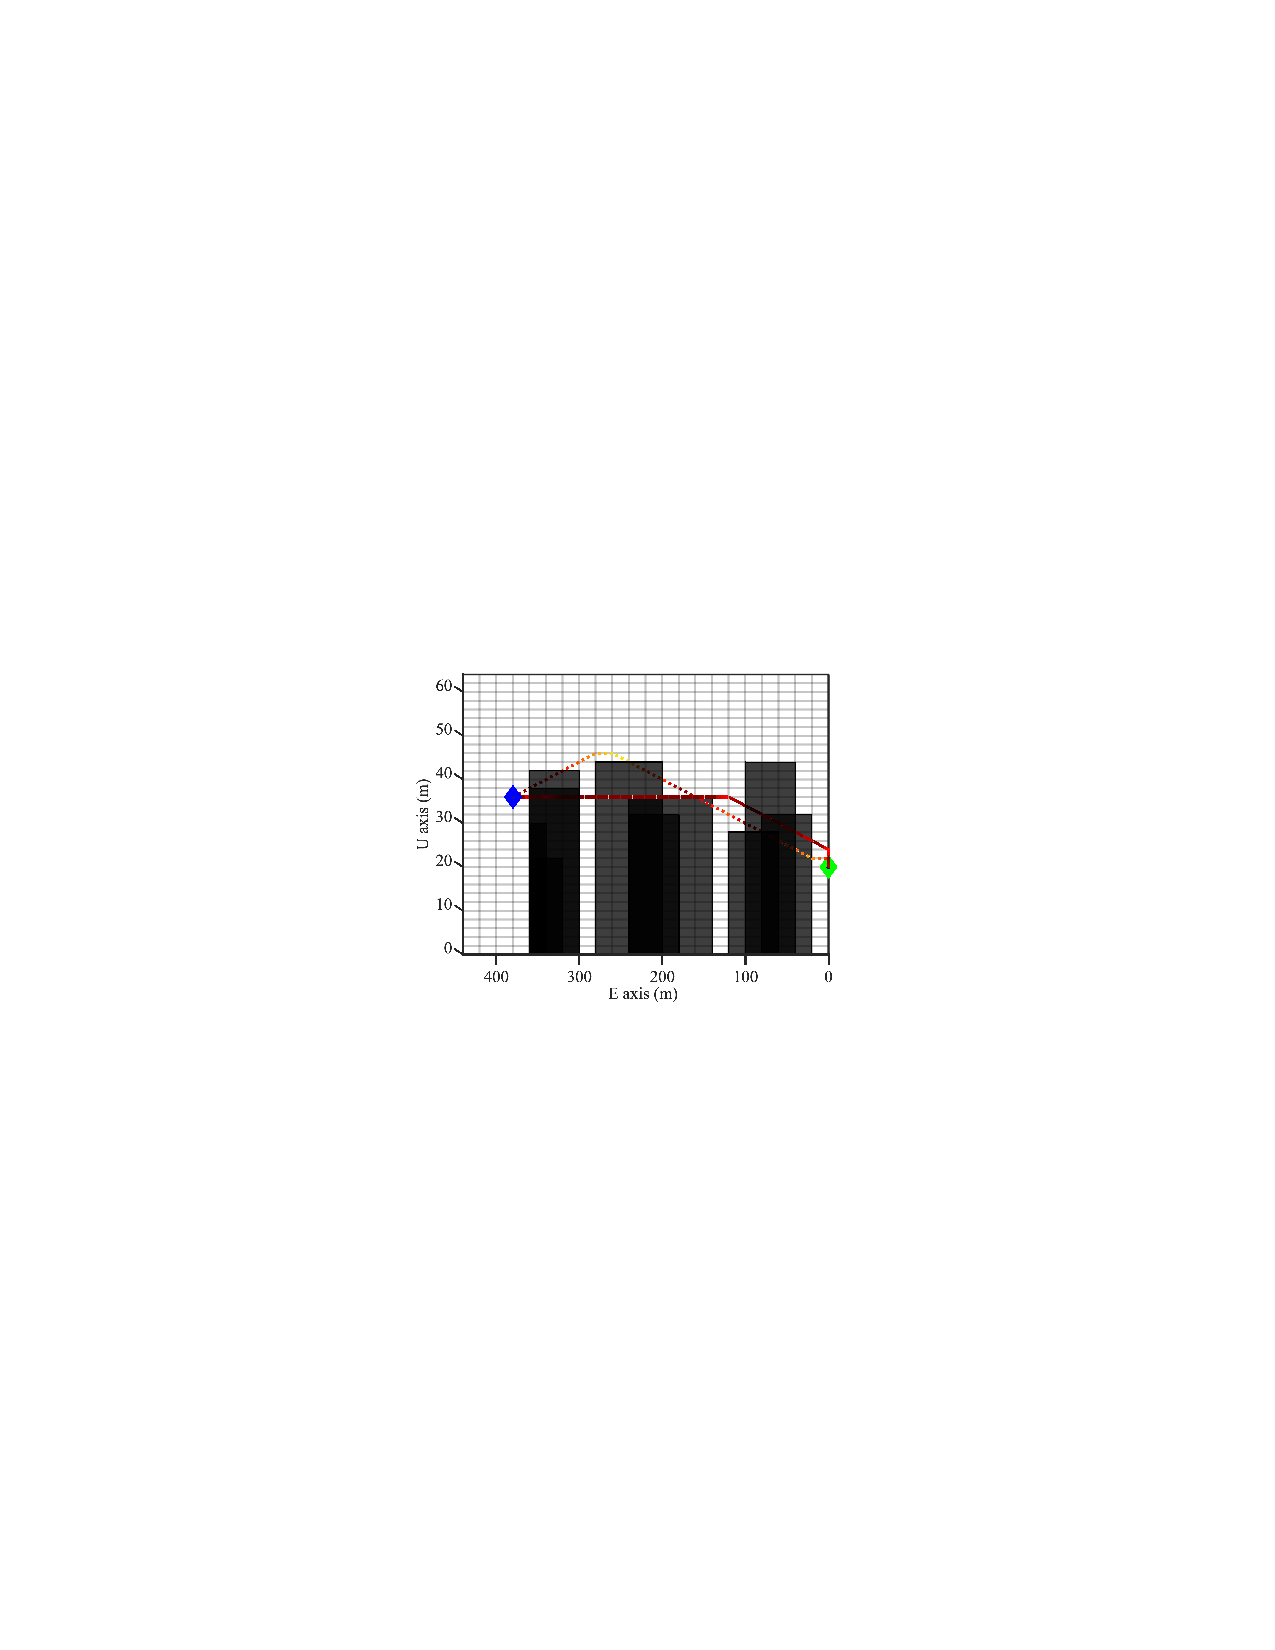
\includegraphics[scale=0.71]{fig15/case1_side.pdf}}
\qquad
\subfloat[The case 2 of the energy minimum path optimization of the drone affected by wind effect.]{\centering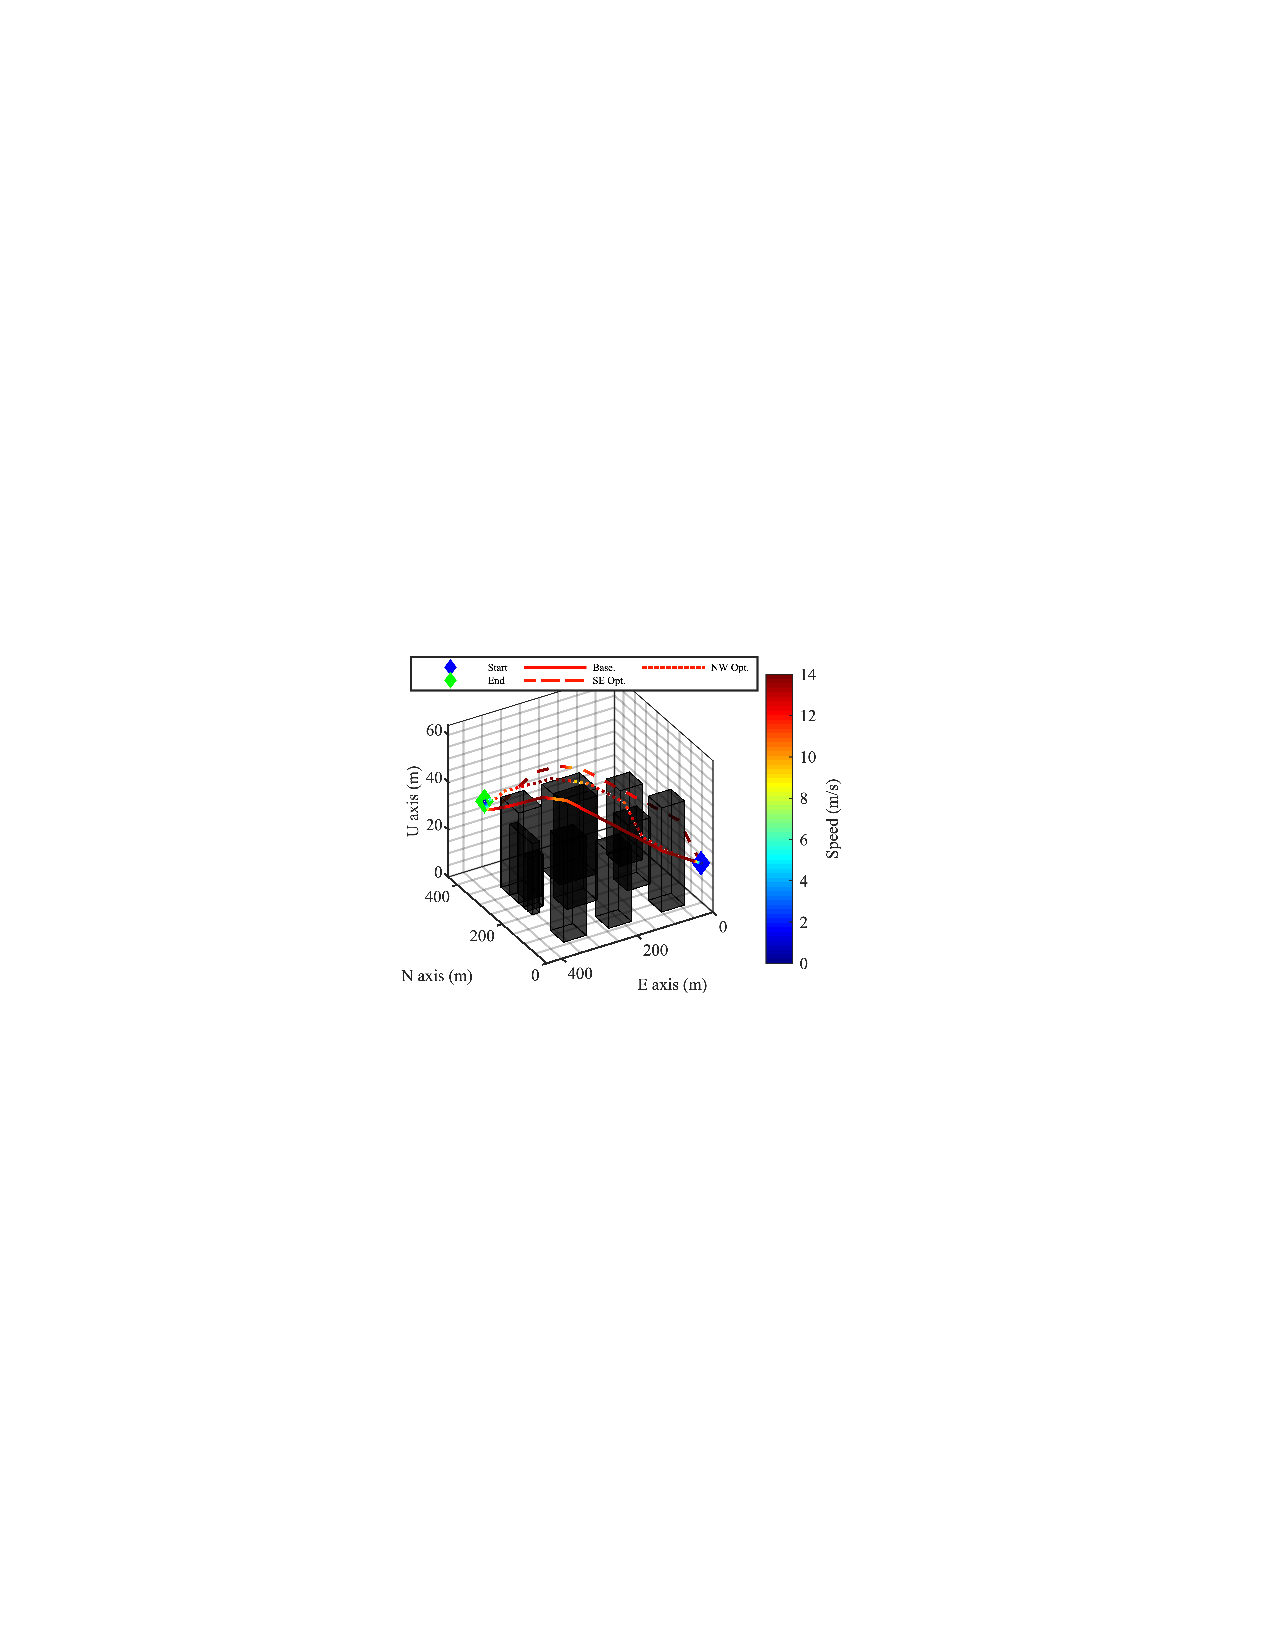
\includegraphics[scale=0.71]{fig15/case2.pdf}}
\subfloat[The top view of case 2.]{\centering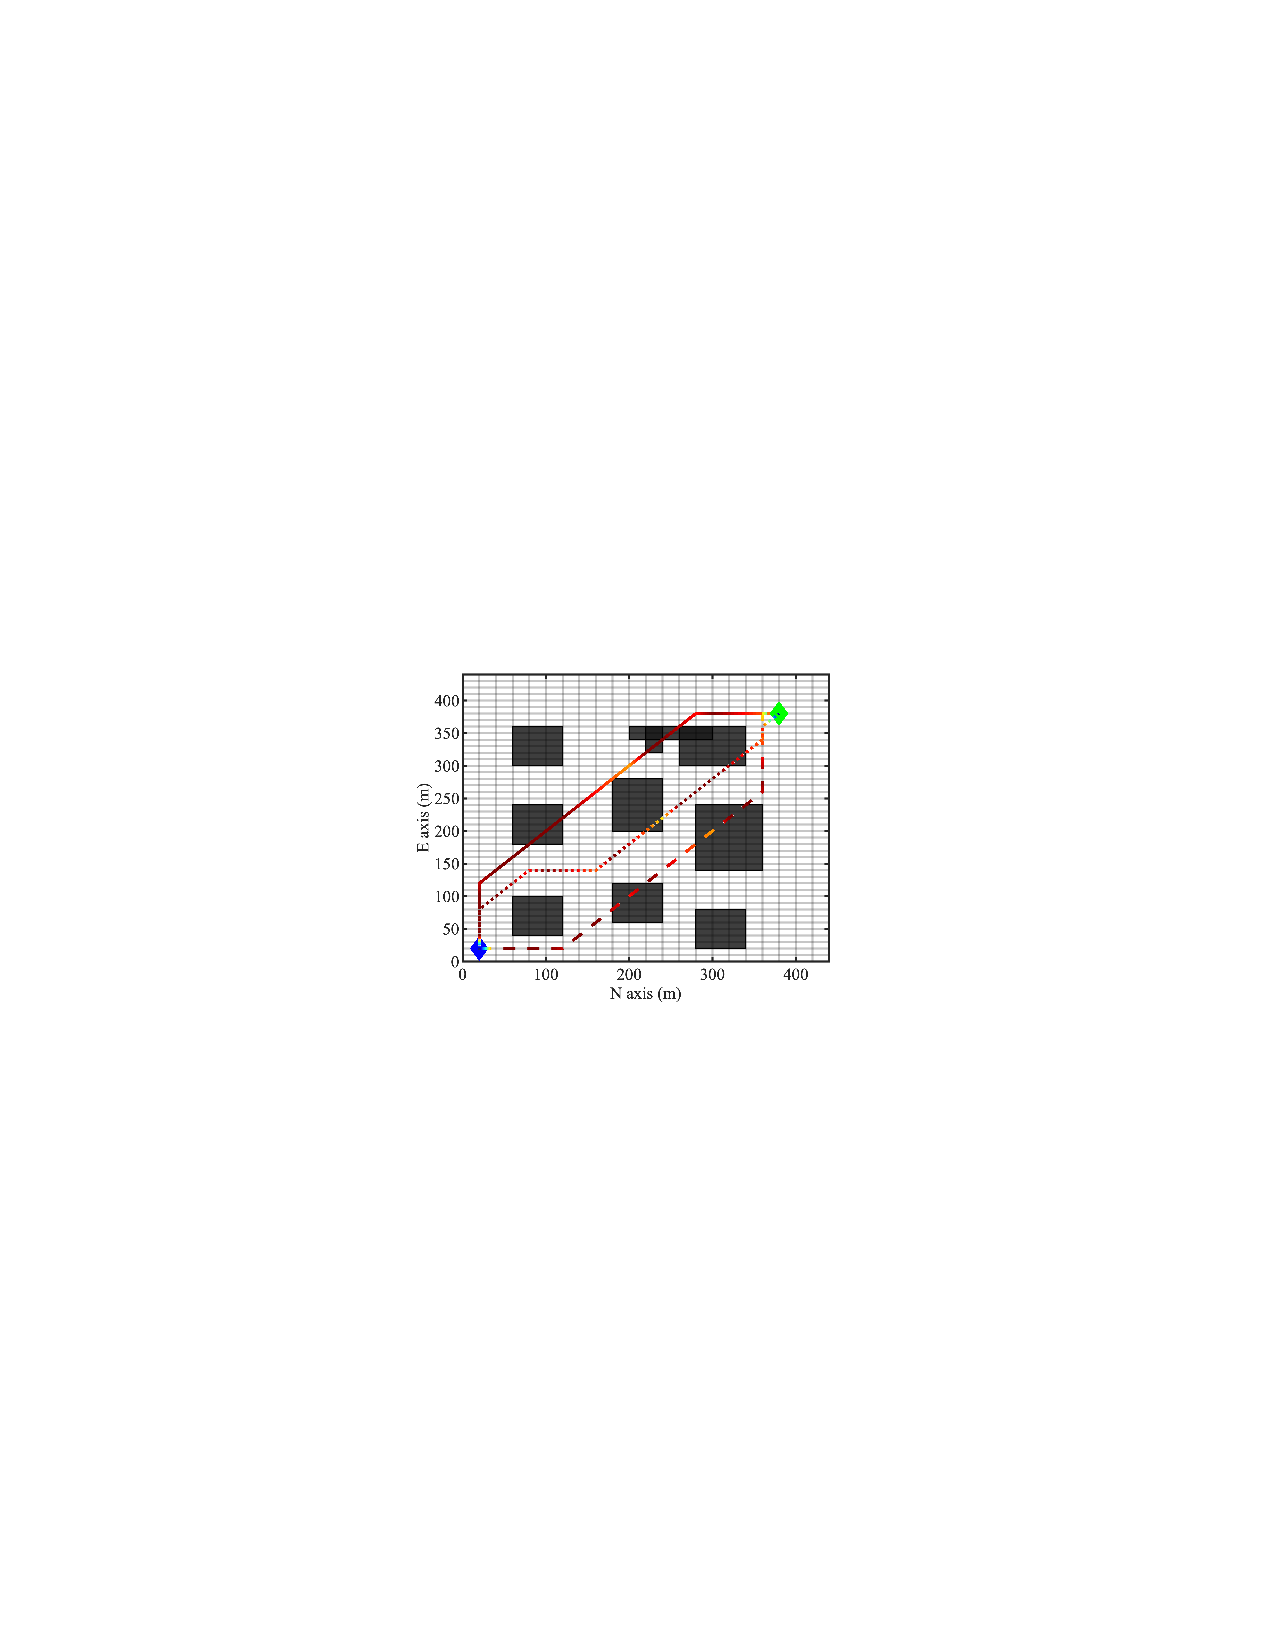
\includegraphics[scale=0.71]{fig15/case2_top.pdf}}
\subfloat[The side view of case 2.]{\centering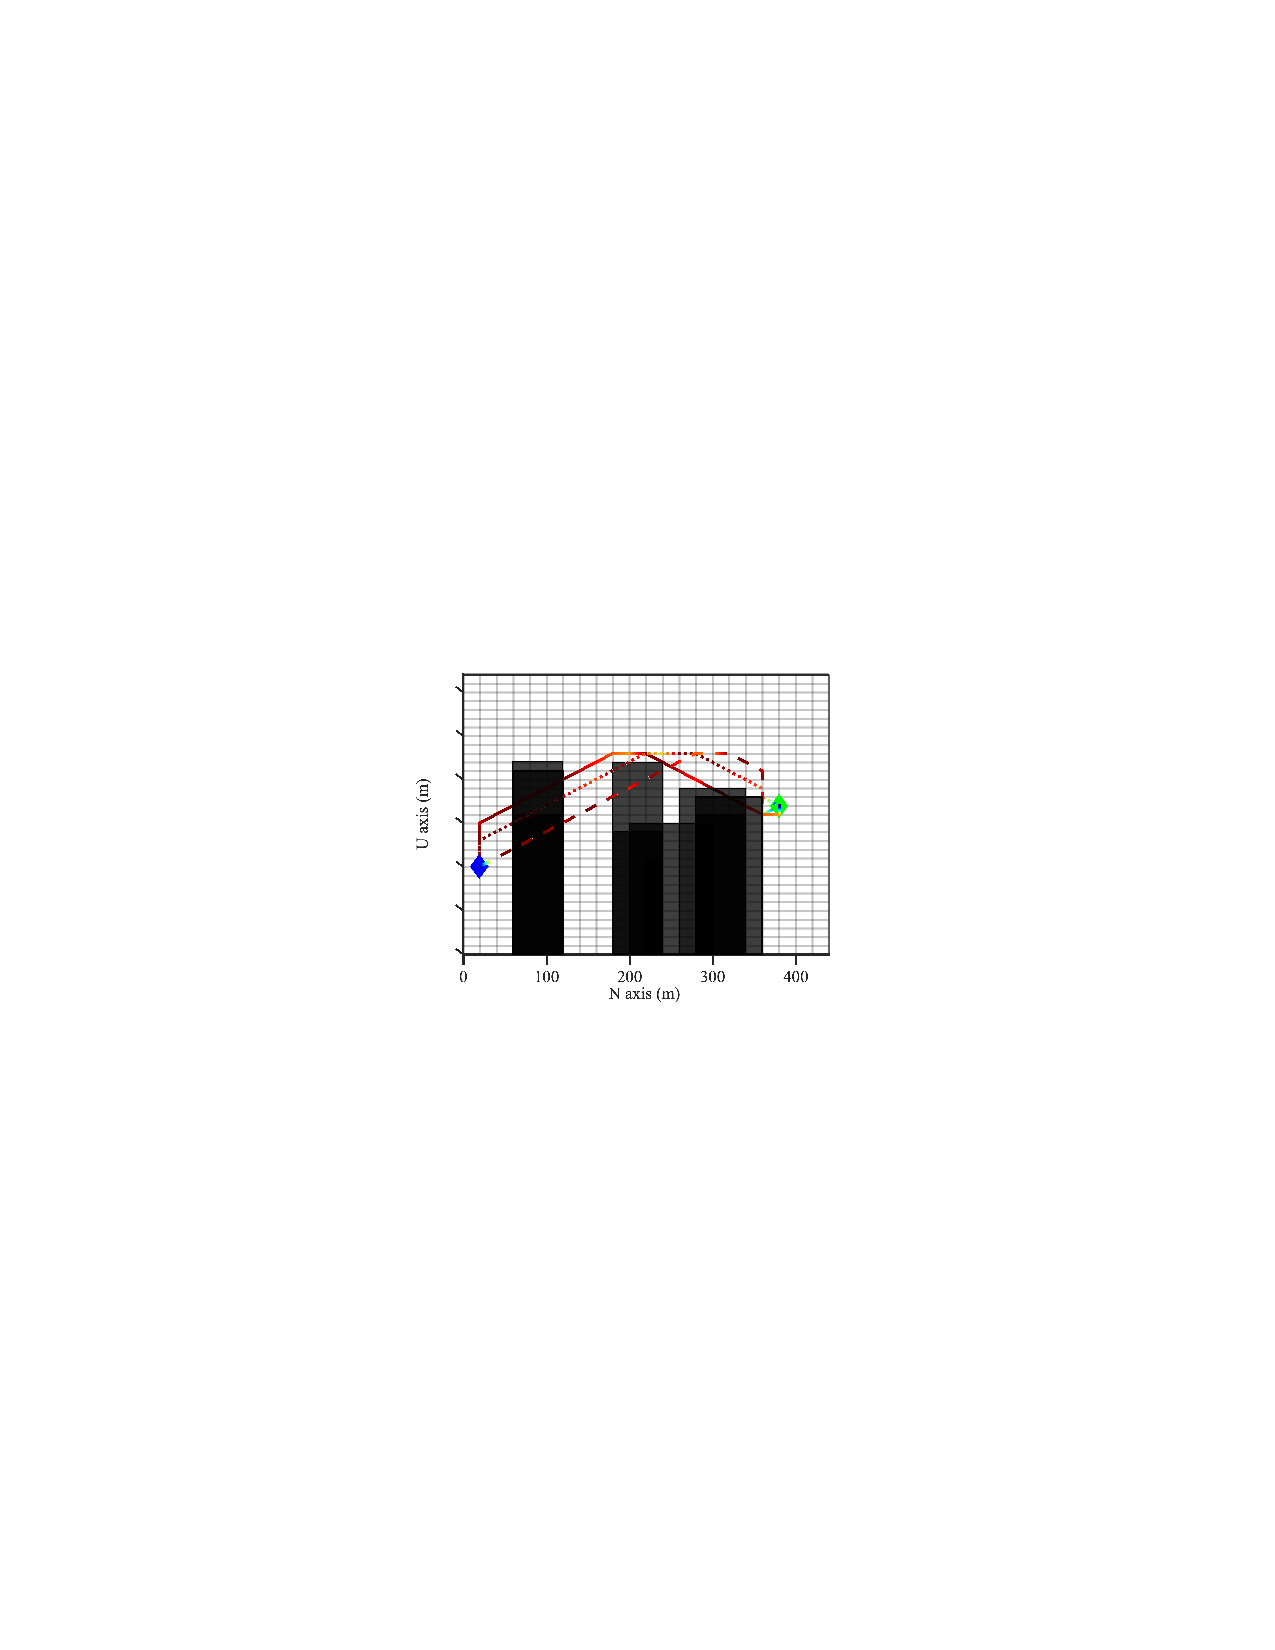
\includegraphics[scale=0.71]{fig15/case2_side.pdf}}
\qquad
\subfloat[The case 3 of the energy minimum path optimization of the drone affected by wind effect.]{\centering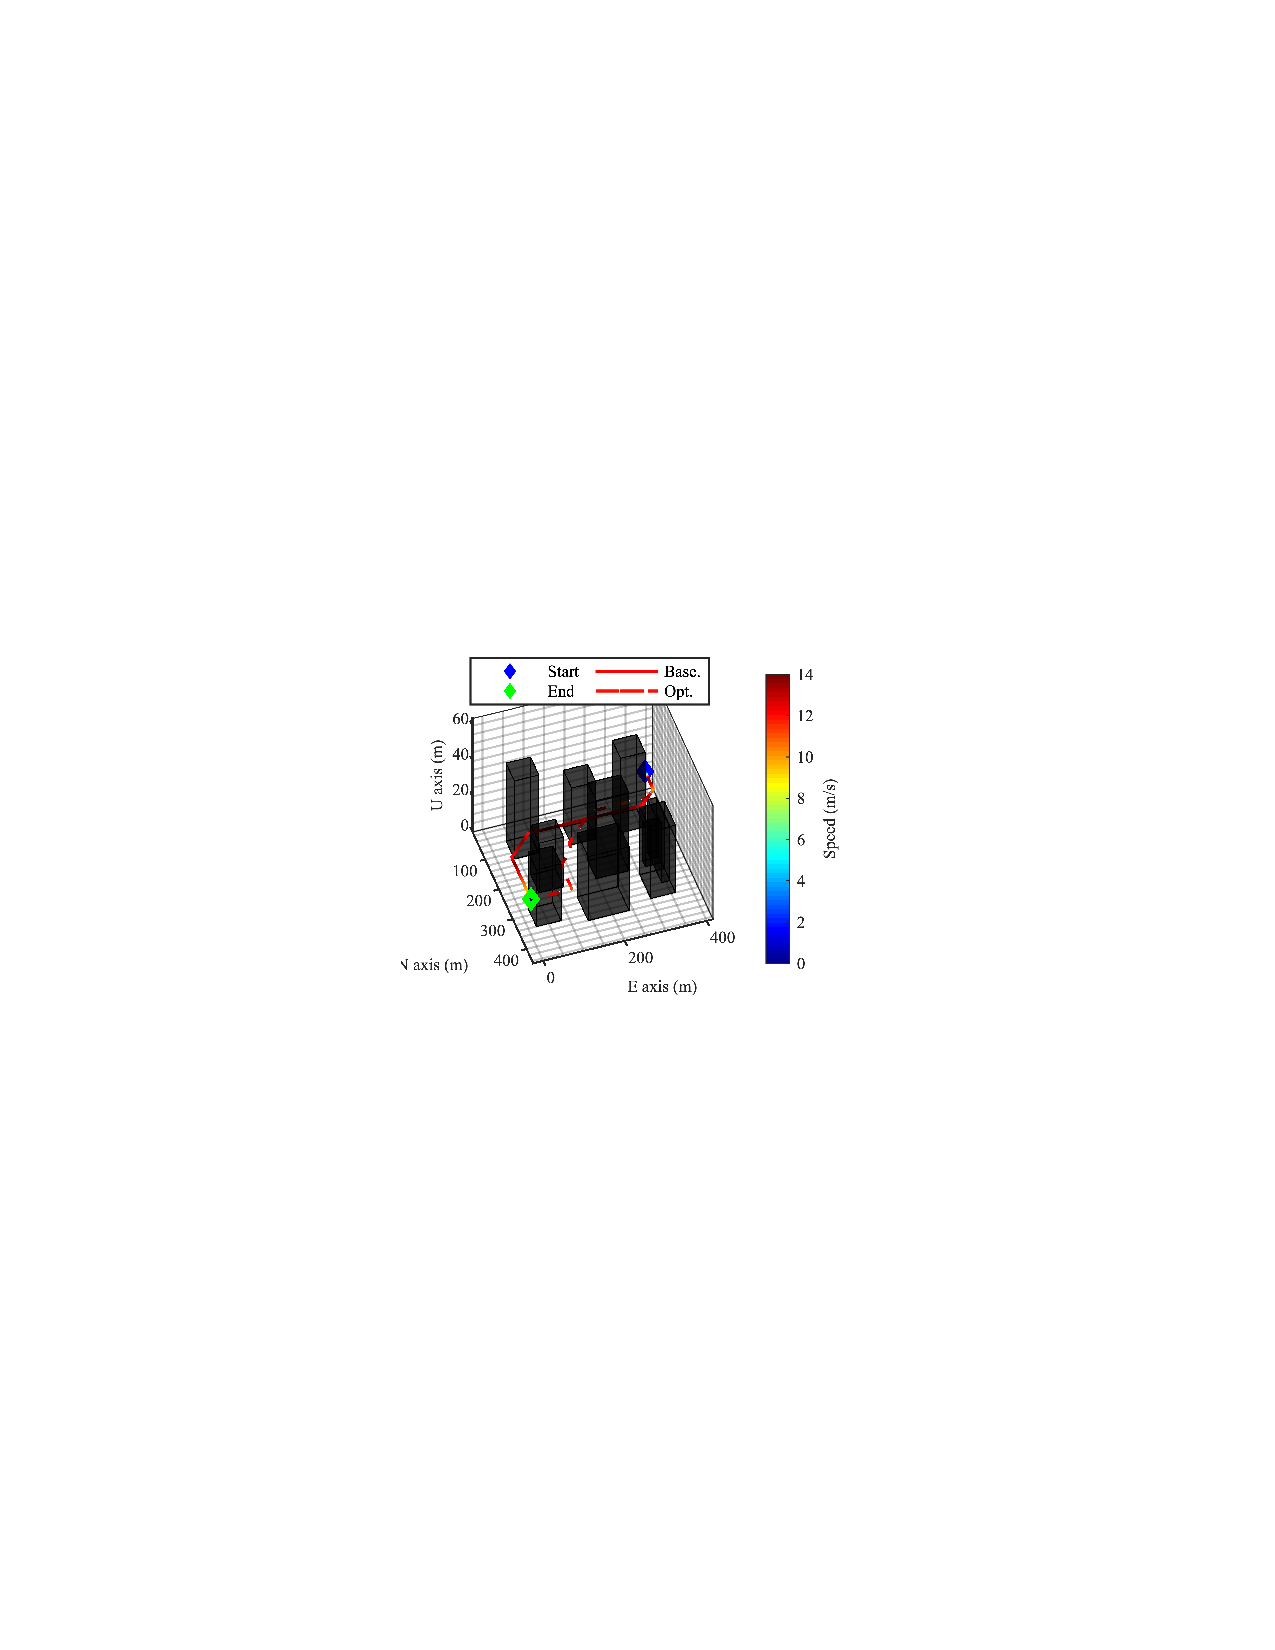
\includegraphics[scale=0.71]{fig15/case3.pdf}}
\subfloat[The top view of case 3.]{\centering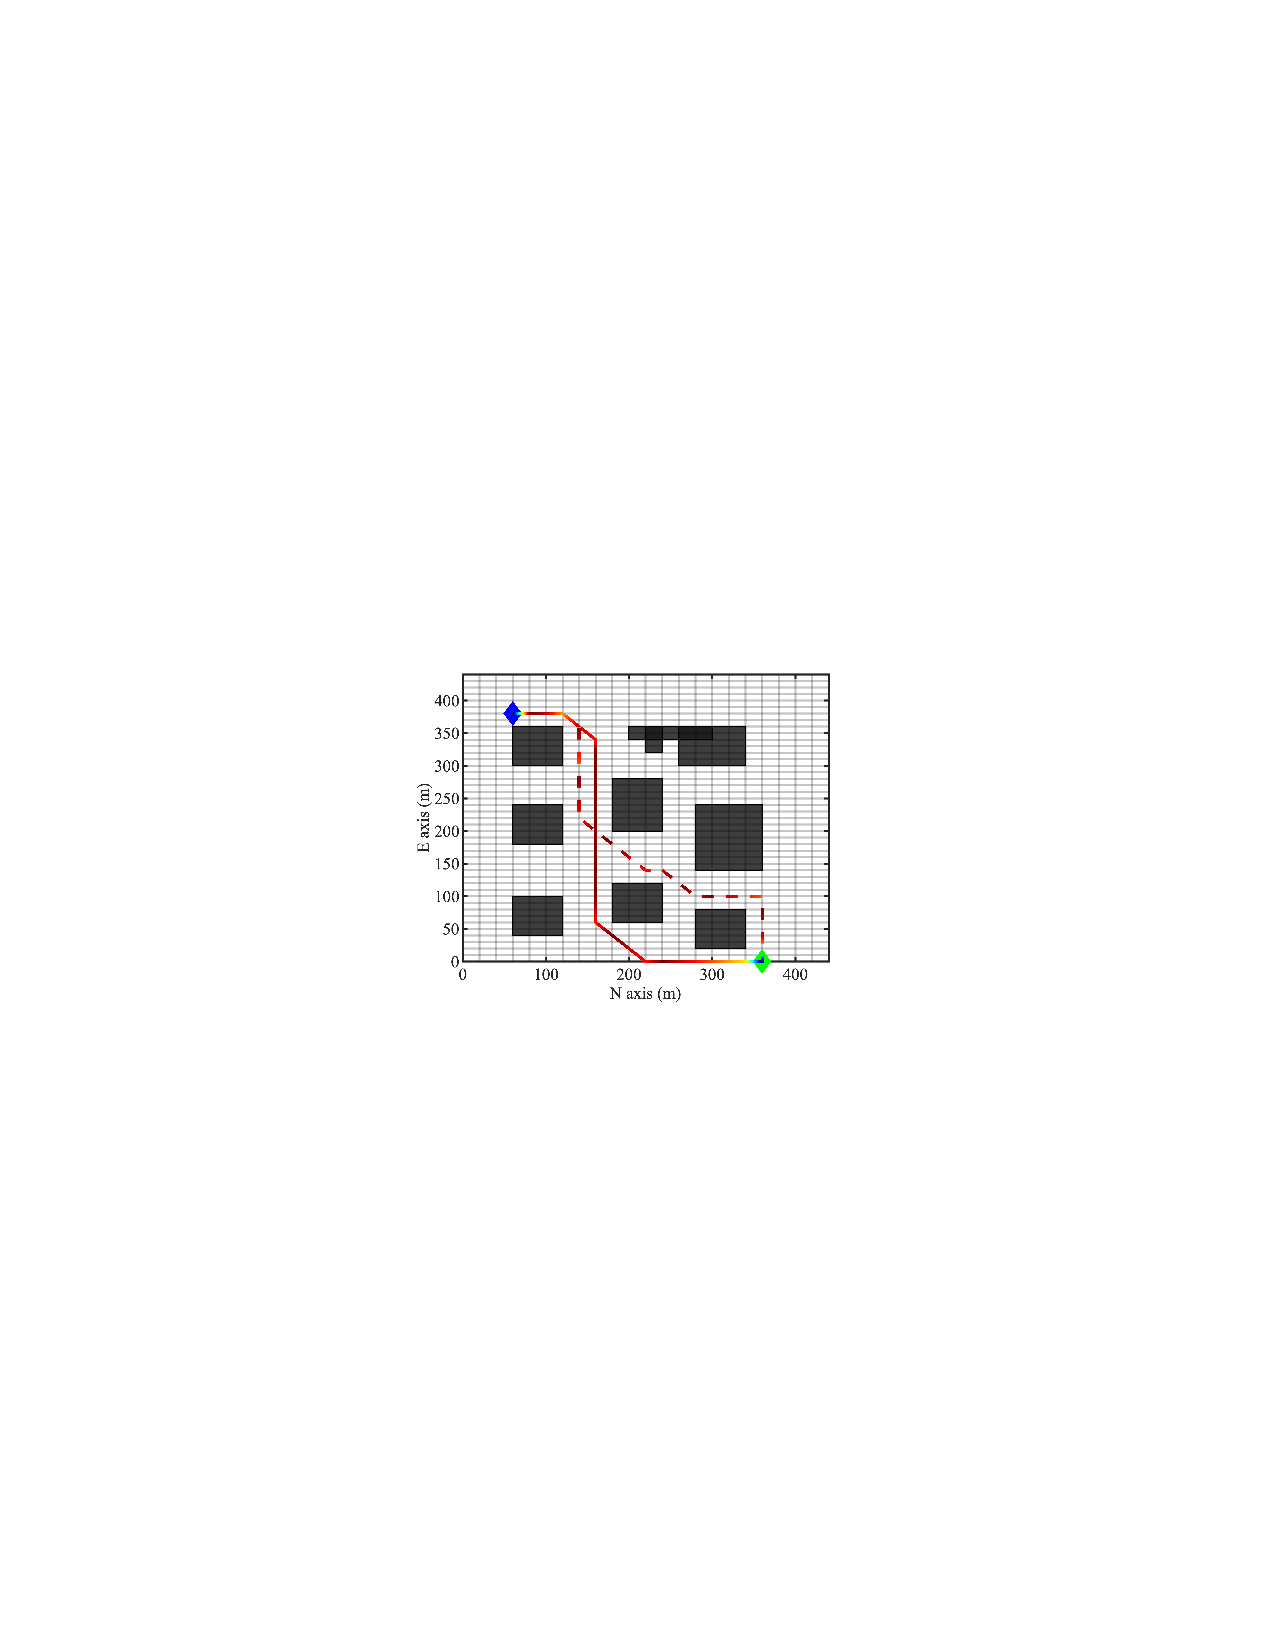
\includegraphics[scale=0.71]{fig15/case3_top.pdf}}
\subfloat[The side view of case 3.]{\centering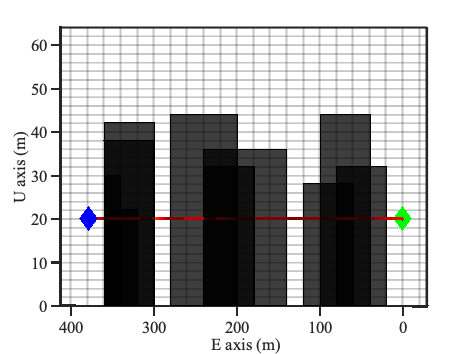
\includegraphics[scale=0.71]{fig15/case3_side.pdf}}
\caption{Each case is under the following conditions: 
(a) Case 1. The wind speed of 6 m/s are applied in the NW and SE directions to the operation environment, respectively. The drone travel in the SE direction between the two points that are at different altitudes.
(b) Case 2. The wind speed of 6 m/s are applied in the NW and SE directions to the operation environment, respectively. but, The drone travel in the SW direction between the two points that are at different altitudes.
(c) Case 3. The wind speed of 6 m/s are applied in the 8 random directions to the operation environment. The drone travel in the SE direction between the two points that are at same altitudes.
}
\label{fig: wind_opt}
\end{figure*}

\noindent In addition, as the power consumption model used for the optimization considers the acceleration, the acceleration and deceleration occurring in the drastic direction of drone change considerably change the speed of the drone, which is different from the energy consumption of the existing baseline.
The comparison result of the consumed energy while going through the generated path with the simulation and the real experiment in Fig.\,\ref{fig:consumed_energy}. 
We perform a measurement to verify the fidelity of the simulation result.
The drone consumes the energy of 48.8\,kJ through the actual flight experiment, and the proposed simulation predicts the energy consumption of 46.1\,kJ.
There is a 5.54\,\% difference between the energy consumption predicted by the proposed simulator and the energy consumed by the real drone.
The validation through the actual flight of the drone shows that the energy consumption deduced by the proposed simulation and the energy consumption of the real drone are not significantly different.
We search the path that the drone consumes the least energy in the environment where the wind effect exists, and compares the energy consumption with the previous optimized path found when there is no existing wind effect.
Unlike when constructing a power consumption model, in the simulation, there is no way to receive wind data in real-time, so we set a constant wind direction and speed in an environment constructed like a weather forecast information.
We present all of the optimization paths in Fig.\,\ref{fig: wind_opt}. 
Fig.\,\ref{fig: wind_opt}(a), (d), and (g) are the optimization cases derived from the flight environment of the drone with different initial conditions. 
The two figures next to each optimization cases are side-view and top-view to identify the changes in the path and the difference in elevation.  
We apply wind speeds of 6\,m/s in the northwest (NW) and southeast (SE) directions in all cases to confirm the optimization results that change with the influence of the wind.
The baseline of each case is a path derived after assuming that there is no wind effect as Fig.\,\ref{fig: opt_environ} and the energy consumption of the baselines are calculated when the drone flies along the baseline applied by the wind direction and speed.

In Fig.\,\ref{fig: wind_opt}(a), the starting point is lower than the ending point, and the drone moves SE direction through the path created. 
When the SE direction wind is applied to the entire environment, the baseline and the optimal path is almost the same.
However, the energy consumption of the two paths differs, the optimal path shows a change in velocity compared to the baseline maintaining the speed based on the translational lift and saves 2.25\,\% energy compared with the baseline.
If the wind in the NW direction is applied, the derived optimal path saves 6.73\,\% of energy compared with the baseline.
Since the wind direction is the reverse direction of the travel, the energy consumption of the drone increases a lot, and the path fluctuates large enough to be intuitively identified, as shown in Fig.\,\ref{fig: wind_opt}(b) and Fig.\,\ref{fig: wind_opt}(c).  
Fig.\,\ref{fig: wind_opt}(d) is a different route with Fig.\,\ref{fig: wind_opt}(a), where the endpoint is higher than the starting point, and the drone moves SW direction.
When the SE wind is applied, the optimal path and baseline show a significant difference of the route; the optimal path is 3.55\,\% efficient than the baseline.
Instead, if the NW wind is applied, the path difference is small, but the length of the path diagonally is long; the optimal path saves 2.23\,\% of energy than the baseline.
The wind effect applied in the side direction of the drone travel causes a change in all optimization paths, with the difference in energy consumption.
Unlike the previous cases, Fig.\,\ref{fig: wind_opt}(g) shows how the optimization path changes when the winds are randomly placed.
Given that random winds affect the flight of the drone, such as the environment in which actual drones operate, the optimal path is more various than when the wind effect is applied in one direction.
The derived optimal path saves 12.7\,\% of energy compared to the baseline. 
Finally, we present the optimization results as Table\,\ref{tab: opt.result} that compares the energy consumption between the baseline and the optimized path affected by wind effect in each case.

\begin{table}[ht]
\caption{Comparison of the energy consumption between the baseline and the optimal path affected by wind effect in each case.}
\label{tab: opt.result}
\resizebox{0.485\textwidth}{!}{%
\begin{tabular}{|c|c|c|c|c|l|l|}
\hline
\multicolumn{1}{|l|}{\multirow{2}{*}{}} & \multicolumn{1}{l|}{\multirow{2}{*}{Wind direction \& speed}} & \multicolumn{2}{c|}{Energy consumption (kJ)} & \multicolumn{3}{l|}{\multirow{2}{*}{Saved energy (\%)}} \\ \cline{3-4}
\multicolumn{1}{|l|}{} & \multicolumn{1}{l|}{} & Baseline & Optimal path & \multicolumn{3}{l|}{} \\ \hline
\multirow{2}{*}{Case 1} & NW (6 m/s)& 41.58 & 40.91 & \multicolumn{3}{c|}{2.25} \\ \cline{2-7} 
& SE (6 m/s)& 62.86 & 58.63  & \multicolumn{3}{c|}{6.73}   \\ \hline
\multirow{2}{*}{Case 2} & NW (6 m/s)& 46.23 & 44.59 & \multicolumn{3}{c|}{3.55}  \\ \cline{2-7} 
& SE (6 m/s)& 50.68 & 49.55 & \multicolumn{3}{c|}{2.23}    \\ \hline
Case 3 & Random (6 m/s)& 52.29 & 45.65 & \multicolumn{3}{c|}{12.7} \\ \hline
\end{tabular}%
}
\end{table}

The results in Table\,\ref{tab: opt.result} show that the results of the drone optimization performed without external force for convenience of calculation in previous studies differed considerably from the actual flight of drones.
Our optimization problem and solution show the maximum benefit from the path derived from the randomly winded environment similar to the actual environments. This has the reliability of deriving a path that consumes the least energy even when the wind direction and speed of reality, which are difficult to apply in the real environment, are applied as simple constants.












\section{Conclusions}

In this paper, we present a systematic framework for optimizing the total operating cost of drones, including accurate power consumption models and optimization methods.
We start from a demonstration that the data provided by the factory onboard power measurement feature of even top-of-the-line commercial drones is highly inaccurate by comparing it with standard equipment. 
This motivates that the power consumption models shown in the previous work may have generated improper predictions compared with the actual power consumption due to the inaccuracy in the measured data.
We implement an accurate in-house onboard power measurement device and collect dozens of hours of power measurement data synchronizing with other flying data. 
Based on the power data, we propose an accurate power consumption model with the deep neural networks. 
The proposed power consumption model exhibits error within 10\,\% compared with a high standard precision data acquisition device. 
The primary benefit of the proposed model is such that i) the model inputs are simple physics parameters of the drone, and external factors affecting power consumption thus it can be easily plugged in various existing optimization framework, and ii) the characterization process is not dependent on the aerodynamics of a particular drone. %iii) considering the three-dimensional velocity and acceleration of the drone at the same time, the power consumption of the drone's momentary movement can easily be predicted.
Finally, we demonstrate a example of energy saving by finding an energy efficient path during the operation of a drone using the proposed accurate power consumption model. The optimal path is derived by accurately considering the wind effects that are generally difficult to consider, and the optimal path is up to 12.7\,\% more energy efficient than the general drone operation for random wind effects.










\section*{Acknowledgment}
This work was supported by the National Research Foundation of Korea (NRF-2018R1A2B3007894) and the 2019 Research Fund of Myongji University. 

\bibliographystyle{unsrt}%Used BibTeX style is unsrt
\bibliography{reference}

\begin{IEEEbiography}[{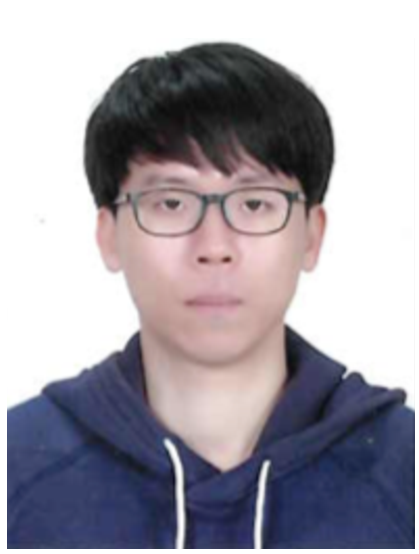
\includegraphics[width=1in,height=1.25in,clip,keepaspectratio]{./bio/dooyoung}}]{Dooyoung Hong}
(S'18) received the B.S. degree in mechanical engineering from Korea University of Technology and Education, Cheonan, Korea in 2017 and received the M.S. degree in the robotics program from Korea Advanced Institute of Science and Technology, Daejeon, Korea in 2019. He is currently pursuing Ph.D. degree in the robotics program, Korea Advanced Institute of Science and Technology. His research interests include low-power embedded system design, and AI based optimization.
\end{IEEEbiography}

\begin{IEEEbiography}[{
\includegraphics[width=1in,height=1.25in,clip,keepaspectratio]{./bio/seonhoon}}]{Seonhoon Lee}
(S'18) received the B.S. degree in electrical engineering from Konkuk University, Seoul, Korea in 2018. He is currently pursuing a master’s degree in the school of electrical engineering, Korea Advanced Institute of Science and Technology. His research interests include low-power embedded system, cyber-physical system, and deep learning.
\end{IEEEbiography}

\begin{IEEEbiography}[{
\includegraphics[width=1in,height=1.25in,clip,keepaspectratio]{./bio/jaemin}}]{Jaemin Kim}
(S'13 M'18) received the B.S. degree in computer science engineering and the M.S. and Ph.D. degrees in computer science and electrical engineering from Seoul National University, Seoul, Korea, in 2005, 2007, and 2018 respectively. He is currently an assistant professor at the department of electronics engineering, Myongji University. His research interests include low-power embedded system design, electrical energy storage system, and energy soruce reconfiguration system.
\end{IEEEbiography}

\begin{IEEEbiography}[{
\includegraphics[width=1in,height=1.25in,clip,keepaspectratio]{./bio/naehyuck}}]{Naehyuck Chang}
(F’12) received the B.S., M.S., and Ph.D. degrees from the Department of Con- trol and Instrumentation, Seoul National Univer- sity, Seoul, South Korea, in 1989, 1992, and 1996, respectively.
From 1997 to 2014, he was at the Department of Computer Science and Engineering, Seoul National University. In 2005, he was a Research Professor at LG Yonam Foundation, Seoul. From 2011 to 2013, he was a Vice Dean of the College of Engineering, Seoul National University. Since 2014, he has been
a Full Professor at the Department of Electrical Engineering, Korea Advanced Institute of Science and Technology, Daejeon, South Korea. He is the Co-Founder of EMVcon, Inc., Irvine CA, USA. His current research interests include low-power cyber-physical systems and design automation of things, such as systematic design and optimization of energy storage systems, electric vehicles, drones, energy harvesting, and so on.
Dr. Chang is a Fellow of the Association for Computing Machinery (ACM) for his contributions to low-power systems. He served as the Chair and the Past Chair for ACM Special Interest Group on Design Automation. He was the TPC Co-Chair of DAC 2016, ASP-DAC 2015, ICCD 2014, CODES+ISSS 2012, ISLPED 2009, and so on, and the General Co-Chair of VLSI-SoC 2015, ICCD 2015 and 2014, ISLPED 2011, and so on. He was a recipient of the 2014 ISLPED Best Paper Award, the 2011 SAE Vincent Bendix Automotive Electronics Engineering Award, the 2011 Sinyang Academic Award, the 2009 IEEE SSCS International SoC Design Conference Seoul Chapter Award, and several ISLPED Low-Power Design Contest Awards in 2002, 2003, 2004, 2007, 2012, 2014, and 2017. He is the Editor-in- Chief of the ACM Transactions on Design Automation of Electronics Systems and serves(ed) as an Associated Editor of the IEEE TRANSACTIONS ON VERY LARGE SCALE INTEGRATION, the IEEE TRANSACTIONS ON COM- PUTER AIDED DESIGN OF INTEGRATED CIRCUITS AND SYSTEMS, the ACM Transactions on Embedded Computing Systems, IEEE EMBEDDED SYSTEMS LETTERS, the IEEE TRANSACTIONS ON CIRCUITS AND SYSTEMS–PART I: REGULAR PAPERS, and so on.
\end{IEEEbiography}


\end{document}
